\chapter{Pattern Avoiding Involutions} 
\label{chap:involutions}

  In this chapter, we investigate sets of pattern-avoiding \emph{involutions}
  \index{involution}. While the enumeration of pattern-avoiding permutations
  has become a major topic of research in recent years, involutions have been
  largely overlooked.  In particular, we focus on finding the Stanley-Wilf
  limit for sets of involutions which avoid patterns of length four. 
  
  Pattern-avoiding involutions were first considered by Simion and
  Schmidt~\cite{Simion1985}, who enumerated the involutions avoiding any length 
  three pattern. As in the case for permutations, the situation quickly becomes
  more complicated for longer patterns. 
  We begin this chapter by examining the simple $123$
  involutions, which will be our primary tool. This chapter is based in part
  on~\cite{me-involutions}. 
  



  
  

% =========================================================================== %
\section{Definitions and Context}
\label{involutions:sec:intro}

  \begin{definition}\label{involutions:def:invclass}
    For a given permutation $\bta$, let $\Av^I(\bta)$ denote the set of
    \emph{$\bta$-avoiding involutions}, the set of involutions (permutations
    which are their own inverse) which do not contain $\bta$. 
    Let $\Av_n^I (\bta)$ be the set of permutations of length $n$ within this set. 
  \end{definition}

  Note that $\Av^I(\bta)$ is not necessarily a \emph{class}, as the set of all
  involutions is not closed under the pattern ordering. However we can apply
  many of the same ideas in order to enumerate these sets.  Clearly, $\Av^I
  (\bta) \subseteq \Av(\bta)$, and so the Marcus-Tardos theorem states that
  each set has a finite upper growth rate. Note that due to the symmetry of
  inversion ($\sg \prec \pi$ if and only if $\sg^{-1} \prec \pi^{-1}$), these
  classes are not principally based in the classical sense. Indeed,
  $\AvnI(\bta) = \AvnI(\bta, \bta^{-1})$ for any permutation $\bta$. For
  simplicity of notation, and to parallel the work done in permutations, we
  write such a set with only a single basis element. 

  \subsection{Previous Results}

    Two patterns $\bta, \tau$ are \emph{involution Wilf-equivalent} if
    $|\AvnI(\bta)| = |\AvnI(\tau)|$. 
    Simion and Schmidt completed the classification of the involution
    Wilf-equivalence classes of patterns of length three in their 1985
    paper~\cite{Simion1985} by showing that, for all patterns $\bta \in
    \{123,132,213,321\}$ and $\sg \in \{231, 312\}$,  
    $$ | \AvnI(\bta)| = \binom{n}{\floor{n/2}} \quad 
          \text{and} \quad |\AvnI(\sg) | = 2^{n-1}.$$

    Extending the work of Guibert, Pergola, and Pinzani~\cite{Guibert2001},
    Jaggard~\cite{Jaggard2002} classified the eight involution Wilf-equivalence
    classes for length four patterns.  Of these classes, only two have been
    successfully enumerated: Gessel~\cite{Gessel1990} counted the set
    $\AvnI(1234)$, while Brignall, Huczynska, and Vatter~\cite{Brignall2008}
    provided the enumeration for $\AvnI(2413)$. In this chapter we enumerate two
    of these unknown sets ($\AvnI(1342)$ and $\AvnI(2341)$), and provide bounds
    for a third ($\AvnI(1324)$). 

    Jaggard~\cite{Jaggard2002} computed the values $|\AvnI(\bta)|$ for each $\bta$
    of length four, up to $n=11$. This data (Table~\ref{involutions:tab:Jaggard})
    suggests an ordering on the eight classes, which we will show is misleading.
    For example, it seems clear from his data that there are more involutions
    avoiding $2341$ than avoiding $1234$. However, there are exponentially more $1234$
    avoiding involutions, as we will soon show. 

    
    \begin{table}[t]
    \caption[The enumeration of involutions avoiding a pattern]{The
              enumerations of involutions avoiding a pattern $\beta$ of length
              $4$ for $n=5$, $\dots$, $11$, as presented by
              Jaggard~\cite{Jaggard2002} (ordered by the last row).}
    \label{involutions:tab:Jaggard}
      $$
      \begin{array}{ccccccccc}%{|c|c|c|c|c|c|c|c|c|}
      &&&&&&&&\\[-10pt]
      &\bm{1324}&\bm{1234}&\bm{4231}&\bm{2431}&\bm{1342}&\bm{2341}&\bm{3421}&\bm{2413}\\[1pt]
      \hline
      &&&&&&&&\\[-11pt]
      |\Av^I_{5}(\beta)|&21&21&21&24&24&25&25&24\\[1pt]
      &&&&&&&&\\[-11pt]
      |\Av^I_{6}(\beta)|&51&51&51&62&62&66&66&64\\[1pt]
      &&&&&&&&\\[-11pt]
      |\Av^I_{7}(\beta)|&126&127&128&154&156&170&173&166\\[1pt]
      &&&&&&&&\\[-11pt]
      |\Av^I_{8}(\beta)|&321&323&327&396&406&441&460&456\\[1pt]
      &&&&&&&&\\[-11pt]
      |\Av^I_{9}(\beta)|&820&835&858&992&1040&1124&1218&1234\\[1pt]
      &&&&&&&&\\[-11pt]
      |\Av^I_{10}(\beta)|&2160&2188&2272&2536&2714&2870&3240&3454\\[1pt]
      &&&&&&&&\\[-11pt]
      |\Av^I_{11}(\beta)|&5654&5798&6146&6376&7012&7273&8602&9600\\[1pt]
      \end{array}
      $$
    \end{table}


  \subsection{Simple Involutions}

    Our primary tool will be the substitution decomposition. Inflations and
    involutions are linked by the following theorem, which provides a recipe
    for constructing new involutions from simples. 

    \begin{theorem}[Brignall, Huczynska, Vatter~\cite{Brignall2008}]
      \label{thm:subsdecomp-inv}
      Let $\sg \neq 21$ be a simple permutation of length $m$, and $\alp_1, 
      \alp_2, \dots \alp_m$. Then $\pi = \sg[\alp_1, \alp_2, \dots \alp_m]$ is
      an involution if and only if $\sg$ is an involution and $\alp_i =
      \alp_{\sg_i}^{-1}$. 
      Further, the skew decomposable involutions are either of the form
      $21[\alp_1, \alp_2]$ with $\alp_1 = \alp_2^{-1}$ or $321[\alp_1, \alp_2,
      \alp_3]$ with $\alp_1 = \alp_3^{-1}$ and $\alp_2 = \alp_2^{-1}$. 
    \end{theorem}

    Describing classes as restricted inflations of their simple permutations is
    a new and useful method for enumerating classes of
    \emph{permutations}~\cite{Albert2012}, and we adapt this method to pattern-avoiding
    \emph{involutions}. As we will show, the simple $2341$-avoiding and
    $1342$-avoiding involutions are (almost) the same as the simple
    $123$-avoiding involutions. The enumerations of these sets can then be
    obtained by appropriately inflating these $123$-avoiding involutions. 

    




\section{Simple 123-Avoiding Permutations}
\label{involutions:sec:perms}

  We step back from involutions briefly, and investigate the simple
  $123$-avoiding \emph{permutations}. This investigation, while interesting on
  its own, provides a gentle introduction to the generating function techniques
  of Section~\ref{involutions:sec:123simples}. In particular, we mirror the
  techniques used by Albert and Vatter~\cite{Vatter2013} to construct and
  analyze a generating function for the $123$-avoiding permutations. 

  \subsection{The Staircase Decomposition}
    
    In Section~\ref{prelim:sec:av123} we investigated the geometric
    structure of the class $\Av 123$, and showed that it contains infinitely
    many simple permutations. While this class is not a grid
    class~\cite{GridClasses}, it can be defined using similar language. The
    \emph{staircase decomposition} of $\Av 123$ allows one to utilize many of
    the specialized techniques which are typically only applicable to grid
    classes, and is central to our study.  

    Every permutation $\pi \in \Av 123$ can be written as a union of two
    increasing sequences of entries (the left-to-right minima and the
    right-to-left maxima). The plot of such a permutation can be fit into a
    \emph{descending staircase} of blocks, the contents of which are monotone
    decreasing. See Figure~\ref{involutions:fig:staircase}. In general, such a
    decomposition is not unique, but for \emph{simple} $123$-avoiding
    permutations we can define a unique gridding as follows: let the first cell
    contain the longest decreasing prefix of the permutation, each eastward
    cell contain all entries whose value is greater than the smallest in the
    previous cell, and each southward cell contain all entries to the left of
    the rightmost entry of the previous cell. 
  
    \begin{figure}[t] \centering
      \begin{tikzpicture}[scale=.25, yscale=-1]
        % draw the outer boxes, using a loop
        \foreach \x/\y in {0/0, 5/0, 5/5, 10/5}{
          \draw[very thick, color=lightgray] (\x, \y) rectangle (\x + 5, \y + 5);
        }
        % closed dots
        \node[closed] at (2,2) {};
        \node[closed] at (4,4) {};
        \node[closed] at (5.6,.6) {};
        \node[closed] at (5.9,5.9) {};
        \node[closed] at (6.2,1.2) {};
        \node[closed] at (7.6,7.6) {};
        \node[closed] at (8.4,3.4) {};
        \node[closed] at (10.5,5.5) {};
        \node[closed] at (12,7) {};
      \end{tikzpicture}
    \caption{The staircase decomposition for the permutation $759381642$.}
    \label{involutions:fig:staircase}
    \end{figure}

    This staircase decomposition was first introduced in~\cite{Albert2010} in
    the study of subclasses of $\Av 321$. As $123$ is the complement of $321$,
    our decomposition is a mirror image of theirs. Note that this decomposition
    separates the left-to-right minima and right-to-left maxima. We will use
    this fact later to build a bivariate generating function that keeps track
    of these entries separately. 

  \subsection{Iterative Process}

    Let $f = \sum_{\pi \in \Av_n 123} x^{n}$. We follow the exposition
    presented by Albert and Vatter in~\cite{Vatter2013} by first giving an
    \emph{almost} correct derivation, then fixing two small errors to obtain
    the correct result. 

    We can build a simple $123$-avoiding permutations iteratively using the
    staircase decomposition by filling one cell at the time. We must, however,
    be careful to ensure simplicity at each step along the way. To this end, we
    fill up an infinite staircase with \emph{filled dots} and \emph{hollow
    dots}; a filled dot represents an entry of the permutation, while a hollow
    dot represents a region which must be filled by at least one entry in order
    to maintain simplicity. Filled dots can be filled with a monotone run of
    entries, but each pair must be \emph{split} by a hollow dot in the next
    cell. Such a diagram with no hollow dots represents a simple $123$-avoiding
    permutations, while a diagram with hollow dots is still a work in progress.
    Since there are only two cells `active' at a time (the current one, and the
    next one), we can represent this process as an iterative system, and our
    goal is then to find a fixed point of the iteration. 

    We build $f$ one cell at a time. At step one, we have a single hollow dot
    in the first cell. At step two, we can fill this hollow dot with a
    descending run of filled dots, but each pair of these necessitates a hollow
    dot in the next cell to split them. During step three, each hollow dot in
    cell two can be filled with a descending run, but again we must place
    hollow dots in cell three to maintain simplicity. See
    Figure~\ref{involutions:fig:perm-iteration} for an example of this
    development. 


    \begin{figure}[t] \centering
        \begin{tikzpicture}[scale=.18, yscale=-1]

          \foreach \x/\y in {0/0}{
            \draw[very thick, color=lightgray] (\x, \y) rectangle (\x + 5, \y + 5);
          }
          \node[open2] at (2.5,2.5) {};
          
        \node at (7.5,2.5) {$\longrightarrow$};

        \begin{scope}[shift={(10,0)}]
          \foreach \x/\y in {0/0, 5/0}{
            \draw[very thick, color=lightgray] (\x, \y) rectangle (\x + 5, \y + 5);
          }
          \node[closed] at (2,2) {};
          \node[closed] at (4,4) {};
          \node[open2] at (6,1) {};
          \node[open2] at (8,3) {};
          \draw[dotted, thick] (3,3)--(7.5,3);
          \draw[dotted, thick] (1,1)--(5.5,1);
        \end{scope}
        
        \node at (22.5,2.5) {$\longrightarrow$};
        
        \begin{scope}[shift={(25,0)}]
          \foreach \x/\y in {0/0, 5/0, 5/5}{
            \draw[very thick, color=lightgray] (\x, \y) rectangle (\x + 5, \y + 5);
          }
          \node[closed] at (2,2) {};
          \node[closed] at (4,4) {};
          \node[closed] at (5.6,.6) {};
          \node[open2] at (5.9,5.9) {};
          \node[closed] at (6.4,1.4) {};
          \node[open2] at (7.6,7.6) {};
          \node[closed] at (8.4,3.4) {};
          \draw[dotted, thick] (5.9,1)--(5.9,5.5);
          \draw[dotted, thick] (7.6,2.6)--(7.6,7.1);
        \end{scope}
        
        \node at (37.5,2.5) {$\longrightarrow$};

        \begin{scope}[shift={(40,0)}]
          \foreach \x/\y in {0/0, 5/0, 5/5, 10/5}{
            \draw[very thick, color=lightgray] (\x, \y) rectangle (\x + 5, \y + 5);
          }
          \node[closed] at (2,2) {};
          \node[closed] at (4,4) {};
          \node[closed] at (5.6,.6) {};
          \node[closed] at (6.1,6.1) {};
          \node[closed] at (6.4,1.4) {};
          \node[closed] at (7.6,7.6) {};
          \node[closed] at (8.4,3.4) {};
          \node[open2] at (10.7,5.7) {};
          \node[open2] at (12,7) {};
          \draw[dotted, thick] (7,7)--(11.5,7);
          \draw[dotted, thick] (5.7,5.7)--(10.2,5.7);
        \end{scope}
        
        \node at (57.5,2.5) {$\longrightarrow$};

        \begin{scope}[shift={(60,0)}]
          \foreach \x/\y in {0/0, 5/0, 5/5, 10/5}{
            \draw[very thick, color=lightgray] (\x, \y) rectangle (\x + 5, \y + 5);
          }
          \node[closed] at (2,2) {};
          \node[closed] at (4,4) {};
          \node[closed] at (5.6,.6) {};
          \node[closed] at (6,6) {};
          \node[closed] at (6.2,1.2) {};
          \node[closed] at (7.6,7.6) {};
          \node[closed] at (8.4,3.4) {};
          \node[closed] at (10.5,5.5) {};
          \node[closed] at (12,7) {};
        \end{scope}

        \end{tikzpicture}
      \caption{The evolution of the permutation $759381642$ by our recurrence.}
      \label{involutions:fig:perm-iteration}
    \end{figure}

    Let $f_i$ be the generating function at stage $i$ of this evolution, with the
    exponent of $x$ indicating the number of filled dots and the exponent of
    $y$ indicating hollow dots (so $f_1 = y$). A hollow dot can be filled with
    a run of filled dots, each pair of which requires a hollow dot, and we have
    the option of placing a new hollow dot above the run. It follows then that
    in each step, each occurrence of $u$ will be replaced by 
    $$ x(1+y) + x^2(y+y^2) + x^3 (y^2 + y^3) + \dots = \frac{x(1+y)}{1-xy}. $$ 
    Thus, we have
    {\small
    $$ f_1(x,y) = y, \quad f_2 
      = f_1\left(x, \frac{x(1+y)}{1-xy}\right) = \frac{x(1+y)}{1 - xy}, \quad 
      f_{i+1} = f_i\left(x, \frac{x(1+y)}{1-xy}\right) \dots .$$
    }

    Since we are interested in permutations with arbitrarily many staircase
    cells, we want to find the limit $f = \limn f_i $. It follows then that $f$
    is a \emph{fixed point} of the iteration $x \ra x; y \ra \frac{x(y+1)}{1 -
    xy}$. Since $f(x,y) = f\left(x, \frac{x(y+1)}{1 - xy}\right)$, can solve
    for $x$ to find
    $$ y = \frac{x(y+1)}{1 - xy} \implies 
       y = \frac{1 - x - \sqrt{1 - 2x - 3x^2}}{2x}.$$

    Thus we have
    $$ \begin{aligned}
      f &= f_1\left(x,\frac{1 - x - \sqrt{1 - 2x - 3x^2}}{2x}\right)\\
        &= \frac{1 - x - \sqrt{1 - 2x - 3x^2}}{2x} \\
        &= x + x^2 + 2x^3 + 4x^4 + 9x^5 + 21x^6 + \dots.
    \end{aligned} $$


    These coefficients are the Motzkin numbers, a well-studied and understood
    sequence (\OEIS{A001006}), but are unfortunately \emph{not} the number of
    simple $123$-avoiding permutations.  This is due to the aforementioned
    errors, which we will now correct. 
    
    
  \subsection{Correcting the Errors}
  \label{involutions:sub:errors}

    Our iteration was correct, but there are some slight discrepancies arising
    in the first two steps of the iteration which must be accounted for. In the
    second step, the `optional' hollow dot above the topmost element is
    actually required, else the permutation will start with its largest entry
    (and therefore not be simple). Furthermore, when this required dot is
    inflated in the third step, the optional dot is in fact forbidden, else we
    will violate the greediness of the gridding. See
    Figure~\ref{involutions:fig:errors} for an illustration. 
    
    

    \begin{figure}[t] \centering
      \begin{tikzpicture}[scale=.3, yscale=-1]
        \foreach \x/\y in {0/0, 5/0}{
          \draw[very thick, color=lightgray] (\x, \y) rectangle (\x + 5, \y + 5);
        }
        \draw[color=white] (-1,-1) -- (10.5,-1) -- (10.5,10.5) -- (-1,10.5) -- cycle;
        \node[closed] at (2,2) {};
        \node[closed] at (4,4) {};
        \node[open2, regular polygon,regular polygon sides=3] at (6,1) {};
        \node[open2] at (8,3) {};
        \draw[dotted, thick] (3,3)--(7.5,3);
        \draw[dotted, thick] (1,1)--(5.5,1);
        \node[white] at (5,10) {};
      \end{tikzpicture}
        \hspace{2pc} 
      \begin{tikzpicture}[scale=.3, yscale=-1]
        \foreach \x/\y in {0/0, 5/0, 5/5}{
          \draw[very thick, color=lightgray] (\x, \y) rectangle (\x + 5, \y + 5);
        }
        \draw[color=white] (-1,-1) -- (10.5,-1) -- (10.5,10.5) -- (-1,10.5) -- cycle;
        \node[closed] at (2,2) {};
        \node[closed] at (4,4) {};
        \node[zball, minimum size=.15cm] at (5.9,5.9) {};
        \node[closed] at (6.4,1.4) {};
        \node[open2] at (7.6,7.6) {};
        \node[closed] at (8.4,3.4) {};
        \draw[dotted, thick] (5.9,1)--(5.9,5.5);
        \draw[dotted, thick] (7.6,2.6)--(7.6,7.1);
      \end{tikzpicture}
      \caption[The hollow triangle represents the location of the hollow dot
                which is required]{
          The hollow triangle represents the location of the hollow dot
          which is required, and the hollow square represents the location of
          the hollow dot which is forbidden.}
    \label{involutions:fig:errors}
    \end{figure}
  
    Fortunately, however, these issues only affect the first three iterations:
    afterwards, the iteration works as initially described. We can therefore
    compensate by simply computing the first three by hand, and then plug in
    the value of $y$ which leads to the fixed point, as found above. 
    As above, we have $f_1 = y$. Since the next optional point is required and
    will be treated differently in the next step, we mark it with a $t$ to
    differentiate it from the standard hollow dots. Thus 
    $$ f_2(x,y,t) = \frac{xt}{1 - xy}.$$
    To compute $f_3$, we perform the standard iteration on the variable $y$,
    and change the variable $t$ into a generating function representing runs of
    filled dots with no option to place one above. This leads to 
    $$ f_3 = f_2 \left( x, \frac{x(y+1)}{1-xy}, \frac{x}{1-xy}\right).$$
  
    At this point the standard iteration, taken to infinity, produces the
    correct generating function, which can be used to enumerate the class $\Av
    (123)$, as shown in Section~\ref{prelim:sec:av123}. 


    \begin{equation} \label{eqn:genfcn-simple123perms}
    \begin{split}
      f(z) &= f_3\left(x, \frac{1 - x - \sqrt{1 - 2x - 3x^2}}{2x}\right) \\
        &= \frac{2x^2}{1 + x^2 + (1+x)\sqrt{1 - 2x - 3x^2}} \\
        &= x^2 + 2x^4 + 2x^5 + 7x^6 + 14x^7 + 37x^8 + \dots.
      \end{split}
    \end{equation}
    The coefficients are \OEIS{A187306}. 



\section{Simple 123-Avoiding Involutions}
\label{involutions:sec:123simples}

  We return now to the problem of enumerating the simple $123$-avoiding
  involutions. Though this is more difficult, the iterative development of the
  generating function for the simple $123$-avoiding permutations presented above
  forms the basis for our study. As we will eventually be inflating these
  involutions to enumerate the avoiding sets, we want to keep track of
  left-to-right minima ($\ltrm$), right-to-left maxima ($\rtlm$), and fixed
  points ($\fp$) separately.  Our goal here will be to find the generating
  functions $s^{(i)}(u,v)$, defined below
  $$ s^{(i)}(u,v) := \sum_{\substack{
            \text{simple } \sg \in \AvnI 123 \\
            \text{with } \fp(\sg) = i }}
            u^{\ltrm(\sg)} v^{\rtlm(\sg)} .$$

    

  \subsection{Extending the Iteration} 

    We proceed defining an iterative process similar to the development
    presented in Section~\ref{involutions:sec:perms}. 
    This iterative process can be extended in a variety of ways, as we will
    soon see. Note, for example, that we could have used a two-part recurrences
    to keep track of the top cells and bottom cells separately; it follows then
    that this process can be used to enumerate the left-to-right minima
    \emph{separately} from the right-to-left maxima with a more technical (but
    no more conceptually difficult) computation. The following sections will
    rely on some tedious and technical calculations, but the core ideas are
    relatively easy to express. 

    Geometrically, an involution is a permutation whose plot is symmetric about
    the line $y = x$ through the plane. As such, we can build a simple
    $123$-avoiding involution using the staircase decomposition \emph{starting
    from the center}, and building out in both directions.
    Figure~\ref{involutions:fig:staircase-center} shows the two possible cases.
    When there is a single fixed point, the case is uniquely determined by
    considering whether the fixed point is a \rtlmax{} or \ltrmin{}. 



    \begin{figure}[t]
    \centering
      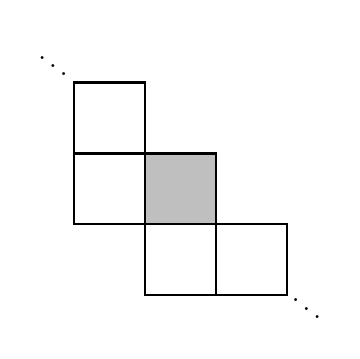
\begin{tikzpicture}[scale=.45]
        \draw[thick,fill=lightgray] (0,0) rectangle (2,2);
        \draw[thick] (-2,0) rectangle (0,2);
        \draw[thick] (0,0) rectangle (2,-2);
        \draw[thick] (-2,2) rectangle (0,4);
        \draw[thick] (2,-2) rectangle (4,0);
        \node at (-2.6,4.7) {$\ddots$};
        \node at (4.55,-2.15) {$\ddots$};
      \end{tikzpicture}
      \hspace{4pc}
      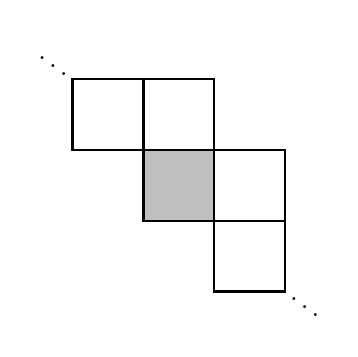
\begin{tikzpicture}[scale=.45,cm={-1,0,0,-1,(0,0)}]
        \draw[thick,fill=lightgray] (0,0) rectangle (2,2);
        \draw[thick] (-2,0) rectangle (0,2);
        \draw[thick] (0,0) rectangle (2,-2);
        \draw[thick] (-2,2) rectangle (0,4);
        \draw[thick] (2,-2) rectangle (4,0);
        \node at (-2.55,4.2) {$\ddots$};
        \node at (4.55,-2.6) {$\ddots$};
      \end{tikzpicture}
      \caption[The diagrams on which we can draw simple permutations]{
        The diagrams on which we can draw simple permutations $\sigma
        \in \Av^I(123)$ that contain a single fixed point.  The starting point
        of the iteration is the shaded cell.}
      \label{involutions:fig:staircase-center}
    \end{figure}
  
    As in Section~\ref{involutions:sec:perms}, we start with a single hollow
    dot in the center cell, and proceed outwards in both directions
    simultaneously while mainaining symmetry. However, the number of fixed
    points determines how we proceed from here. In the interest of clarity, we
    develop the single fixed point case in detail, and give a sketch of the
    details of the other cases. 

  \subsection{Single Fixed Point}
 

    We first develop the generating function $\htso(z) = s^{(1)}(z,z)$, which
    only keeps track of the number of such permutations of each length and
    ignores the ltr-min and rtl-max, and then indicate how to obtain the
    more general $\htso(u,v)$. The set of all simple $(123)$-avoiding
    involutions with exactly one fixed point can be partitioned based on
    whether the fixed point is a ltr-min or a rtl-max. These two sets are
    in bijection with each other, as mapping a permutation to its reverse
    complement maps one set to the other. Therefore it suffices to enumerate
    those in which the fixed point is a rtl-max, and then simply double the
    result to obtain the full generating function (or in the case of $s^{(1)}$,
    add the result to itself with the rtl-max and ltr-min switched). 
  
    Assume that the fixed point is a rtl-max. The first hollow dot must then
    be inflated by an odd number of filled dots (with the fixed point at the
    center). The hollow dots here behave a bit differently than in the previous
    section: each pair of filled dots can be split either below or to the left,
    or both. Of these possible splittings, one of them (see
    Figure~\ref{involutions:fig:bad-case} yields a skew decomposable
    permutation, violating the simplicity condition. We can account for this
    with a calculation which takes the symmetry into account. 

    \begin{figure}[t]
    \centering
      \begin{tikzpicture}[scale=.15]
        % draw the outer boxes, using a loop
        \foreach \x/\y in {-10/0, 0/0, 0/-10}{
          \draw[very thick, color=lightgray] (\x, \y) rectangle (\x + 10, \y + 10);
        }
        % dotted line through diagonal
        \draw[dotted] (-9,-9) -- (11,11);

        % closed dots
        \foreach \i in {-4, -2, 0, 2, 4}{
          \node[closed] at (5-\i,5+\i) {};
        }
        % open dots
        \foreach \i in {1,3}{
          \node[open] at (-5-\i, 5+\i) {};
          \draw[color=gray] (-4.5-\i,5+\i) -- (5.5-\i, 5+\i);
        }
        \foreach \i in {-1,-3}{
          \node[open_y] at (5-\i, -5+\i) {};
          \draw[color=gray] (5-\i,-4.5+\i) -- (5-\i, 5.5+\i);
        }
      \end{tikzpicture}
    \caption[An example of a bad placement]{
        An example of a bad placement of splitting entries that leads to
        a skew decomposable permutation.} 
    \label{involutions:fig:bad-case}
    \end{figure}


    Suppose that the initial cell (which contains the fixed point) contains a total
    of $2k+1$ entries. It follows that $k$ of these entries lie below and to the
    right of the fixed point. Because $\sigma$ is simple, each of the $2k$ adjacent
    pairs of entries in this cell must be separated by entries in the cell below,
    by entries in the cell to the left, or by both types of entries. Each adjacent
    pair lying above and to the left of the fixed point has a corresponding
    adjacent pair (its image under inversion) which lies below and to the right of
    the fixed point; if we split the former to the left, then the inverse-image of
    the separating entry splits the latter below, and vice versa.

    We can split each adjacent pair with as few as $k$ entries in the cell below
    the fixed point, and this can be done in $2^k$ ways by picking which of each
    two corresponding pairs of entries to split below. Similarly, the number of
    ways to have $k+i$ separating entries in the cell below is given by $2^{k-i}{k
    \choose i}$, since we can first pick which of the $i$ corresponding pairs of
    gaps between entries are split both to the left and below, then we choose which
    of each of the remaining $k-i$ corresponding pairs are split below or to the
    left.

    As in the derivation in Section~\ref{involutions:sub:errors}, there are a
    few slight difficulties we must take into account, but again they only
    arise in the first three steps of the iteration. We therefore construct
    these three steps by hand, before letting the iteration go to infinity. 

    Every choice of separating entries leads to a simple permutation except
    one: if we split all of the pairs of entries to the right of the fixed point by
    entries below the initial cell and split no other pairs, then the resulting
    permutation will be skew decomposable, as shown in
    Figure~\ref{involutions:fig:bad-case}. We compensate for these ``bad cases'' by
    subtracting the term $x/(1 - x^2y)$. 



    It follows that
    $$ \begin{aligned}
      \htso_2(x,y,z)
      &=
      \frac{2z}{y}\left(\sum_{k=0}^\infty \left(x^{2k+1}\sum_{i=0}^k
          2^{k-i}{k\choose i}y^{k+i}\right) - \frac{x}{1-x^2y}\right)\\ 
      &=
      \frac{2x^3z(1+y)}{(1-x^2y)(1-2x^2y-x^2y^2)}.
    \end{aligned} $$
    % s2 := 2*z*(x^2*y + x^2) / (x^4*y^3 + (2*x^4 - x^2)*y^2 - 3*x^2*y + 1);



    \begin{figure}[t]
      \centering
      \begin{tikzpicture}[scale=.15]

        % draw the outer boxes, using a loop
        \foreach \x/\y in {0/0}
        \draw[very thick, color=lightgray] 
        (\x, \y) -- (\x + 10, \y) -- (\x + 10, \y + 10) -- (\x, \y + 10) -- cycle;
        % dotted line through diagonal
        \draw[dotted] (0,0) -- (10,10);

        % draw the center y dot
        \node[open_y] at (5,5) {};
        \node[fill=none] at (5,-12.5) {$s^{(1)}_1$};
      \end{tikzpicture}
      %
      \hspace{2em}
      %
      \begin{tikzpicture}[scale=.15]
        % draw the outer boxes, using a loop
        \foreach \x/\y in {-10/0, 0/0, 0/-10}
        \draw[very thick, color=lightgray] 
        (\x, \y) -- (\x + 10, \y) -- (\x + 10, \y + 10) -- (\x, \y + 10) -- cycle;
        % dotted line through diagonal
        \draw[dotted] (-9,-9) -- (11,11);

        % closed dots
        \foreach \i in {-4, -2, 0, 2, 4}{
          \node[closed] at (5-\i,5+\i) {};
        }
        % open dots
        \foreach \i in {1,3}{
          \node[open] at (-5-\i, 5+\i) {};
          \draw[color=gray] (-4.5-\i,5+\i) -- (5.5-\i, 5+\i);
        }
        \foreach \i in {-1,-3}{
          \node[open_y] at (5-\i, -5+\i) {};
          \draw[color=gray] (5-\i,-4.5+\i) -- (5-\i, 5.5+\i);
        }
        \node[zball] at (2,-2) {};
        \node[zball] at (-2,2) {};
        \draw[color=gray] (2,-1.5) -- (2, 8.5);
        \draw[color=gray] (-1.5,2) -- (8.5,2);

        \node[fill=none] at (5,-12.5) {$s^{(1)}_2$};
      \end{tikzpicture}
      %
      \hspace{2em}
      %
      \begin{tikzpicture}[scale=.15] % s3
        % draw the outer boxes, using a loop
        \foreach \x/\y in {-10/10, -10/0, 0/0, 0/-10, 10/-10}
        \draw[very thick, color=lightgray] 
        (\x, \y) -- (\x + 10, \y) -- (\x + 10, \y + 10) -- (\x, \y + 10) -- cycle;
        % dotted line through diagonal
        \draw[dotted] (-9,-9) -- (18,18);

        % closed dots
        \foreach \i in {-4, -2, 0, 2, 4}{
          \node[closed] at (5-\i,5+\i) {};
        }
        \foreach \i in {1,-3.3,-2.7, 2.7,3.3}{
          \node[closed] at (-5-\i, 5+\i) {};
        }
        \foreach \i in {2.7,3.3, -1,-2.7, -3.3}{
          \node[closed] at (5-\i, -5+\i) {};
        }

        % open dots
        \foreach \i in {-3, 3}{
          \draw[color=gray] (14.5-\i, -4.8+\i) -- (5.3-\i, -4.8+\i);
          \draw[color=gray] (-4.8+\i, 14.5-\i) -- (-4.8+\i, 5.3-\i);
          \node[open_y] at (15-\i, -4.8+\i) {};
          \node[open] at (-4.8+\i, 15-\i) {};
        }
        % extra open dot
        \draw[color=gray] (14.5,-5) -- (5.5, -5);
        \draw[color=gray] (-5,14.5) -- (-5, 5.5);
        \node[open_y] at (15,-5) {};
        \node[open] at (-5,15) {};
        \node[fill=none] at (5,-12.5) {$s^{(1)}_3$};
      \end{tikzpicture}
    \caption{Three stages of the recurrence, in the case when the single
            fixed point is a right-to-left maximum.}
    \label{involutions:fig:3stages}
    \end{figure}


    The $2$ in $\htso_2$ accounts for both cases, where the fixed point is a
    \rtlmax{} and a \ltrmin{}, while the $z/y$ factor counts the topmost
    hollow dot in the cell below the fixed point by $z$ instead of $y$, as it
    will require special care. By our definition of greediness, this topmost
    hollow dot, shown as a hollow square in
    Figure~\ref{involutions:fig:3stages}, is not allowed to produce an
    hollow dot above it in the next cell. Therefore, when substituting for $z$ to
    obtain $\htso_3$, we substitute $x^2/(1-x^2y)$ instead of
    $x^2(1+y)/(1-x^2y)$. As such, we obtain


    $$ \htso_3(x,y)
        =s_2\left(x, \frac{x^2(1+y)}{1-x^2y}, \frac{x^2}{1-x^2y}\right). $$
    % s3 := subs({y = x^2*(1+y) / (1 - x^2*y), z = x*(1 - x^2*y)}, s2);

    After this point, the same iteration leads from $\htso_i$ for $\htso_{i+1}$
    for all $i \geq 3$. Since the filled dots above the center cell are
    completely determined by those below, we need only consider the expansion
    of hollow dots in the bottom cell. Their expansion is exactly as in
    Section~\ref{involutions:sec:perms}, except that each expansion of a hollow
    dot adds dots in both the bottommost cell and the topmost. Letting $i \geq
    3$, this leads to the relation
    \begin{equation}\label{involutions:eqn:iteration-inv}
      \htso_{i+1}(x,y) = \htso_i \left(x, \frac{x^2(y+1)}{1-x^2y} \right).
    \end{equation}

    To find the limit of this iteration, it suffices to find at fixed point,
    and plug it in for $y$ in the expression $\htso_3(x,y)$. 
    This leads to 
    \begin{equation} \label{involutions:eqn:htso}
      \begin{split}
      \htso(x) 
      &= \htso_3 \left(x, \frac{1 - x^2 - \sqrt{1-2x^2 - 3x^4}}{2x^2}\right) \\
      &= \frac{2x^5 \left(1 + x^2 + \sqrt{1 - 2x^2-3x^4}\right)}{%
          (1+x^2)^2 \left(1 - 3x^2 + (1-2x^2)\sqrt{1-2x^2-3x^4}\right)} \\
      &= 2x^5 + 2x^7 + 10x^9 + 22x^{11} + 68x^{13} + 184x^{15} + 530x^{17}
      +\dots \\
      \end{split}
    \end{equation}

    Note that an involution with only a single fixed point is necessarily of
    odd length, and so the power series in equation~\ref{involutions:eqn:htso}
    contains no terms with even powers. 


    Rather than repeat this full derivation to find $\sone(u,v)$, we simply
    indicate the changes to make to the above calculation.  Recall that $u$
    (resp. $v$) represents a filled dot which is a ltr-min (reps. rtl-max), and
    introduce new variables $y_u$ and $y_v$ which represent hollow dots which
    are ltr-min and rtl-max, respectively.  We can assume that the fixed point
    is a rtl-max, because then we can just add this generating function to
    itself with the $u$ and $v$ swapped to obtain the full generating function
    $\sone(u,v)$. 

    A hollow dot in a lower cell, represented by $y_u$, then leads to filled
    dots in the lower cell (represented by $u$) and hollow dots in an upper
    cell (represented by $y_v$s).  A similar description of hollow dots in an
    upper cell leads to the iterations
    \begin{equation}\label{involutions:eqn:dual-iterations}
      \begin{split}
      y_u &\mapsto \frac{u^2 (1 + y_v)}{1 - u^2 y_v} \\ 
      y_v &\mapsto \frac{v^2 (1 + y_u)}{1 - v^2 y_u}.
      \end{split}
    \end{equation}

    To find the fixed point of this iteration, we can compute two iterations
    and solve. That is, solve for $y_v$ in the expression 

    $$ \begin{aligned} 
        y_v &=  \frac{v^2 (1 + y_u)}{1 - v^2 y_u} \\
        &= \frac{v^2 \left(1 + \frac{u^2 (1 + y_v)}{1 - u^2 y_v}\right)}{%
          1-v^2 \frac{u^2 (1 + y_v)}{1 - u^2 y_v}} \\
        &= \frac{v^2 (1 + u^2}{%
            1 - u^2v^2 - u^2y_v - u^2v^2y_v}. 
    \end{aligned} $$

    Solving this system yields the fixed point of the iteration: 
    \begin{equation} \label{involutions:eqn:dualfixed}
      y_v = \frac{1 - u^2v^2 - \sqrt{1 - 6u^2v^2 - 4u^2v^4 - 
                                     4u^2v^2 - 3u^4v^4}}{%
                  2u^2(1+v^2)}.
    \end{equation}

    Mirroring the construction of $\htso$, we can derive
    $\sone_3(u,v,y_u, y_v)$ by hand using these extra variables. Note that
    there will be no $y_u$ terms in this expression, because at the third stage
    the only hollow dots will be in cells corresponding to left-to-right
    minima. The limit of the iteration is then given by plugging in the fixed
    point to this expression. This gives the generating function for the case
    when the fixed point is a rtl-max, but by swapping occurrences of $u$ and
    $v$ and then adding it back to itself, we obtain the full generating
    function $\sone$. 

    {\small
    \begin{equation} \label{involutions:eqn:sone}
      \begin{split}
      \sone(u,v) &= 
        \frac{u^2v^3(1+u^2)(1+2v^2+u^2v^2+r)}
        {(1+v^2)(1-6u^2v^2-4u^2v^4-4u^4v^2-3u^4v^4+(1-3u^2v^2-2u^4v^2)r)}\\
        &\text{where} \quad r := \sqrt{1-6u^2v^2-4u^2v^4-4u^4v^2-3u^4v^4}.
      \end{split}
    \end{equation}
    }


  \subsection{Zero and Two Fixed Points}
  \label{involutions:sub:02fp}
    
    We now turn to the remaining two cases, in which the involution has no
    fixed points or two fixed points. The derivation is largely the same as the
    single fixed point case, so we simply sketch the changes that must be made. 
    Each of these has their own idiosyncrasies, but they can be dealt with
    easily. 

    First, consider the case of involutions with no fixed points. Such a
    permutation cannot be uniquely gridded, because the diagonal line on which
    the fixed points would lie can be taken to pass through either a lower or
    upper central cell. It follows, however, that every involution with no
    fixed points can be decomposed in both ways, and so it suffices to assume
    that the diagonal line passes through an upper cell, and take this to be
    our initial cell. 

    Since there is no fixed point, this initial cell must have an even number
    of elements. We build the first three iterations by hand, in the same
    manner as the one fixed point case, before substituting the fixed point of
    the iteration. A similar bad case (Figure~\ref{involutions:fig:bad-case})
    must be accounted for, and the same restriction applies to the topmost
    hollow dot of the second cell, as shown in
    Figure~\ref{involutions:fig:3stages}. 

    The generating function $\htsz$ enumerating the class according to length, and the
    corresponding bivariate generating function $\szero$ enumerating the
    ltr-min and ltr-max entries are given below. 

    {\small
    \begin{equation} \label{involutions:eqn:htszero}
      \begin{split}
      \htsz(x) &=
      \frac{2x^6(1+x^2-\sqrt{1-2x^2-3x^4})}{2-2x^2-10x^4-6x^6+(2-6x^4-4x^6)\sqrt{1-2x^2-3x^4}}\\
      % s := (2*x^6 + 2*x^8 - 2*x^6*sqrt(1-2*x^2-3*x^4)) /
      % (2-2*x^2-10*x^4-6*x^6+(2-6*x^4-4*x^6)*sqrt(1-2*x^2-3*x^4))
      &= x^8+2x^{10}+8x^{12}+22x^{14}+68x^{16}+198x^{18}+586x^{20}+\cdots.
      \end{split}
    \end{equation}

    \begin{equation} \label{involutions:eqn:szero}
      \begin{split}
      \szero(u,v)
      &= \frac{2u^2v^4(1+u^2)(1+2u^2+u^2v^2-r)}
      {(1-u^2v^2+r)(1-6u^2v^2-4u^2v^4-4u^4v^2-3u^4v^4+(1+2v^2+u^2v^2)r)} \\
        &\text{where} \quad r := \sqrt{1-6u^2v^2-4u^2v^4-4u^4v^2-3u^4v^4}.
      \end{split}
    \end{equation}
    }


    Finally, we consider the case of involutions with two fixed points. As with
    the case of no fixed points, such a permutation can be drawn on either of
    the two diagrams shown in Figure~\ref{involutions:fig:staircase}. To ensure
    uniqueness, break our own rules slightly to say that the topmost fixed
    point is the center of the initial cell, while the bottom fixed point lies
    on the southwest corner of this cell. See
    Figure~\ref{involutions:fig:twofix} for an example, and note that in this
    case, the hollow square is allowed to produce a hollow dot above itself in
    the next cell, as this no longer violates the greediness of the
    decomposition (because of the lower fixed point). 

    
    \begin{figure}[t]
      \centering
      \begin{tikzpicture}[scale=.15]

        % draw the outer boxes, using a loop
        \foreach \x/\y in {0/0}
        \draw[very thick, color=lightgray] 
        (\x, \y) -- (\x + 10, \y) -- (\x + 10, \y + 10) -- (\x, \y + 10) -- cycle;
        % dotted line through diagonal
        \draw[dotted] (0,0) -- (10,10);

        % draw the center y dot
        \node[open_y] at (5,5) {};
        \node[closed] at (0,0) {};
        \node[fill=none] at (5,-12.5) {$s^{(1)}_1$};
      \end{tikzpicture}
      %
      \hspace{2em}
      %
      \begin{tikzpicture}[scale=.15]
        % draw the outer boxes, using a loop
        \foreach \x/\y in {-10/0, 0/0, 0/-10}
        \draw[very thick, color=lightgray] 
        (\x, \y) -- (\x + 10, \y) -- (\x + 10, \y + 10) -- (\x, \y + 10) -- cycle;
        % dotted line through diagonal
        \draw[dotted] (-9,-9) -- (11,11);
        \node[closed] at (0,0) {};

        % closed dots
        \foreach \i in {-4, -2, 0, 2, 4}{
          \node[closed] at (5-\i,5+\i) {};
        }
        % open dots
        \foreach \i in {1,3}{
          \node[open] at (-5-\i, 5+\i) {};
          \draw[color=gray] (-4.5-\i,5+\i) -- (5.5-\i, 5+\i);
        }
        \foreach \i in {-1,-3}{
          \node[open_y] at (5-\i, -5+\i) {};
          \draw[color=gray] (5-\i,-4.5+\i) -- (5-\i, 5.5+\i);
        }
        \node[zball] at (2,-2) {};
        \node[zball] at (-2,2) {};
        \draw[color=gray] (2,-1.5) -- (2, 8.5);
        \draw[color=gray] (-1.5,2) -- (8.5,2);

        \node[fill=none] at (5,-12.5) {$s^{(1)}_2$};
      \end{tikzpicture}
      %
      \hspace{2em}
      %
      \begin{tikzpicture}[scale=.15] % s3
        % draw the outer boxes, using a loop
        \foreach \x/\y in {-10/10, -10/0, 0/0, 0/-10, 10/-10}
        \draw[very thick, color=lightgray] 
        (\x, \y) -- (\x + 10, \y) -- (\x + 10, \y + 10) -- (\x, \y + 10) -- cycle;
        % dotted line through diagonal
        \draw[dotted] (-9,-9) -- (18,18);
        \node[closed] at (0,0) {};

        % closed dots
        \foreach \i in {-4, -2, 0, 2, 4}{
          \node[closed] at (5-\i,5+\i) {};
        }
        \foreach \i in {1,-3.3,-2.7, 2.7,3.3}{
          \node[closed] at (-5-\i, 5+\i) {};
        }
        \foreach \i in {2.7,3.3, -1,-2.7, -3.3}{
          \node[closed] at (5-\i, -5+\i) {};
        }

        % open dots
        \foreach \i in {-3, 3}{
          \draw[color=gray] (14.5-\i, -4.8+\i) -- (5.3-\i, -4.8+\i);
          \draw[color=gray] (-4.8+\i, 14.5-\i) -- (-4.8+\i, 5.3-\i);
          \node[open_y] at (15-\i, -4.8+\i) {};
          \node[open] at (-4.8+\i, 15-\i) {};
        }
        % extra open dot
        \draw[color=gray] (14.5,-5) -- (5.5, -5);
        \draw[color=gray] (-5,14.5) -- (-5, 5.5);
        \node[open_y] at (15,-5) {};
        \node[open] at (-5,15) {};
        \node[fill=none] at (5,-12.5) {$s^{(1)}_3$};
      \end{tikzpicture}
    
    \caption{The decomposition of an involution with two fixed points.} 
    \label{involutions:fig:twofix}
    \end{figure}

    Note also that the `bad case' (Figure~\ref{involutions:fig:bad-case}) is no
    longer a bad case, as the lower fixed point maintains simplicity. Also, we
    are now allowed to add a hollow dot in the second cell immediately to the
    right of the lower fixed point, as long as we insert a hollow dot above
    this entry in the third cell. Taking these factors into consideration, we
    have the following generating functions for $\htsz$ and $\szero$. 

  \begin{equation} \label{involutions:eqn:htstwo}
    \begin{split}
    \htsz(x)
    &=
    \frac{x^4(2+5x^2+3x^4-(2+x^2)\sqrt{1-2x^2-3x^4})}
    {1-x^2-5x^4-3x^6+(1+2x^2+x^4)\sqrt{1-2x^2-3x^4}}\\
    &=
    3x^6+4x^8+15x^{10}+36x^{12}+105x^{14}+288x^{16}+819x^{18}+\cdots.
    \end{split}
  \end{equation}

	% s := (2*x^4+5*x^6+3*x^8-(2*x^4+x^6)*sqrt(1-2*x^2-3*x^4)) / (1-x^2-5*x^4-3*x^6+(1+2*x^2+x^4)*sqrt(1-2*x^2-3*x^4));
  \begin{equation} \label{involutions:eqn:stwo}
    \begin{split}
    \szero(u,v)
    &= \frac{uv^3\pa{2+7u^2+4u^2v^2+4u^4+3u^4v^2-(2+u^2)r}}
    {1-6u^2v^2-4u^2v^4-4u^4v^2-3u^4v^4+(1+2v^2+u^2v^2)r} \\
    &\text{where} \quad r := \sqrt{1-6u^2v^2-4u^2v^4-4u^4v^2-3u^4v^4}.
    \end{split}
  \end{equation}
    

  We can now combine the generating functions $\szero, \sone, \stwo$ to obtain
  a generating function for all simple $123$-avoiding permutations, enumerated
  by number of left-to-right minima and right-to-left maxima. However, it will
  be convenient to keep these separate, because in the next section we will
  explore inflations of these permutations, and oftentimes fixed points have
  different inflation rules from other entries. 
       
      




\section{Enumerating Pattern Avoiding Involutions}
\label{involutions:sec:enumerations}
  
  We are now in position to enumerate the sets $\Av^I(1342)$ and $\Av^I(2341)$.
  Our tool for both of these is to first show that the simples in each set
  (almost) coincides with the simples within $\Av^I(123)$. This allows us to
  describe each of these sets by inflations of these simples, and so we need
  only determine what inflations are allowed to enumerate the sets. 


  \subsection{Involutions Avoiding 1342}
  \label{involutions:sub:1342}

    Clearly, every involution avoiding $1342$ must also avoid $1342^{-1} =
    1423$. We first show that the set of simples in this set are precisely
    the $123$-avoiding simple involutions. This will be easy once we establish
    suitable notation. 

    \begin{definition} \label{involutions:def:subs-closure}
      Given a permutation class $\C$, define its \emph{substitution closure}
      $\vect{\C}$ to be the largest class with the same simple permutations as
      $\C$. 
    \end{definition}

    By definition, since $\Av(123) \subseteq \Av(1342, 1423)$, we have that
    the $123$-avoiding simples are contained in $\Av(1342, 1423)$.
    Atkinson, Ru\v{s}kuc, and Smith~\cite{Atkinson2011} investigated
    substitution closures, and found that 
    $$ \vect{\Av(123)} = \Av(24153, 25314, 31524, 41352, 246135, 415263).$$
    Each of these basis elements contains either $1342$ or $1423$, and so we
    have the following relation and its consequences. 
    $$ \Av(1342, 1423) \subseteq \vect{\Av(123)}.$$ 

    \begin{proposition} \label{involutions:prop:1342simpleperms}
      The simple permutations within $\Av(1342, 1423)$ are precisely the same
      as the simple permutations within $\Av(123)$. 
    \end{proposition}

    \begin{corollary} \label{involutions:cor:1342simple}
      The simple involutions within $\Av(1342, 1423)$ are precisely the same
      as the simple involutions within $\Av(123)$. 
    \end{corollary}

    To enumerate the set we now need only describe the allowable inflations
    which maintain pattern avoidance and involutionicity. We divide the simples
    into three classes: first we have the inflations of $1$, which themselves
    must be simple. Then come the inflations of $12$ and $21$, the sum- and
    skew-decomposable permutations, respectively. Finally we consider
    inflations of simples of length greater than three. 



    We begin by by defining $f$ to be the generating function for the class
    $\Av(1342,1423)$ and $f_\oplus$ (resp., $f_\ominus$) the generating
    function for the sum (resp., skew) decomposable permutations of this class.
    We then define $g$ to be the generating function for the set $\Av^I(1342)$
    and $g_\oplus$ (resp., $g_\ominus$) the generating function for the sum
    (resp., skew) decomposable $1342$-avoiding involutions.

    
    First we describe the sum decomposable permutations
    $\pi=\alpha_1\oplus\alpha_2$ counted by $g_\oplus$. By
    Proposition~\ref{thm:subsdecomp}, we can assure uniqueness of
    decomposition by requiring that $\alpha_1$ is sum indecomposable. To produce
    an involution, $\alpha_1$ and $\alpha_2$ must be involutions as well. In
    order for $\pi$ to avoid the patterns $1342$ and $1423$, it is required that
    $\alpha_1$ avoids these patterns, and that $\alpha_2$ avoids the patterns
    $231$ and $312=231^{-1}$.

    In fact, the class $\Av(231,312)$, known as the class of \emph{layered
    permutations}, consists entirely of involutions because a permutation lies in
    $\Av(231,312)$ if and only if it can be expressed as a sum of some number of
    decreasing permutations. The layered permutations of length $n$ are in
    bijection with compositions of $n$, and hence there are $2^{n-1}$
    permutations of length $n$ in $\Av(231,312)$. Therefore, $g_\oplus$ satisfies
    the equation 
    
    $$ g_\oplus = \pa{g - g_\oplus}\pa{\frac{x}{1-2x}}. $$

    From this expression it follows that

      \begin{equation}
      \label{involutions:eqn:1342-1}
      g_\oplus = \frac{gx}{1-x}.
      \end{equation}

    Next we must briefly consider the permutation class $\Av(1342,1423)$.
    Kremer~\cite{Kremer2000, KremerPS} showed that
    this class is counted by the large Schr\"oder numbers, \OEIS{A006318}, and
    has generating function 
    $$ f(x) = \frac{1-x-\sqrt{1-6x+x^2}}{2}. $$
    Since this permutation class is skew closed (because both $1342$ and $1423$
    are skew indecomposable), it follows by Proposition~\ref{thm:subsdecomp}
    that, since 
    $f_\ominus = (f - f_\ominus)f$ and $f_\ominus = \frac{f^2}{1+f}$, 

    $$ f - f_\ominus = \frac{f}{1+f} = \frac{1+x-\sqrt{1-6x+x^2}}{4}. $$

    This is the generating function for the \emph{small} Schr\"oder numbers,
    \OEIS{A001003}. 


    Returning our attention to $\Av^I(1342)$, which is also skew closed, we
    note that skew indecomposable permutations in this set are of the form
    $\alpha_1\ominus\alpha_2\ominus\alpha_1^{-1}$ where $\alpha_1$ is a skew
    decomposable member of $\Av(1342,1423)$ and $\alpha_2$ is an arbitrary (and
    possibly empty) member of $\Av^I(1342)$. Therefore we see that

    \begin{equation}
      \label{involutions:eqn:1342-2}
      g_\ominus = \pa{f(x^2)-f_\ominus(x^2)}(1+g).
    \end{equation}
      
    Lastly, we must enumerate $1342$-avoiding involutions which are inflations of
    simple permutations of length at least four. Any such simple permutation must
    have at least two right-to-left maxima and by simplicity every right-to-left
    maximum must have some entry both below it and to the left. Hence to avoid
    creating a copy of $1342$ or $1423$, we may only inflate right-to-left maxima
    by decreasing intervals. An entry which is a left-to-right minimum can be
    inflated by any permutation in the class $\Av(1342,1432)$. However, to ensure
    that the inflated permutation is an involution, we must inflate each fixed
    point by an involution. Additionally, if we inflate the entry with value
    $\sigma(i)$ by the permutation $\alpha$, we must make sure to inflate the
    entry with value $i$ by $\alpha^{-1}$.

    Consider $s^{(0)}(u,v)$, which is the generating function for
    simple involutions of length at least four which avoid $123$ and have zero
    fixed points. To inflate each right-to-left maximum by a decreasing
    permutation in a way that yields an involution, we substitute 
    
    $$ v^2 = \frac{x^2}{1-x^2} .$$

    This follows because if $\sigma(i)$ is a right-to-left maximum of the simple
    $123$-avoiding involution $\sigma$ then the entry with value $i$ will also be
    a right-to-left maximum, and we must substitute a permutation and its inverse
    into this pair of entries of $\sigma$. Because the class $\Av(1342,1423)$ is
    counted by the large Schr\"oder numbers, the inflations of the simple
    involutions of length at least four with zero fixed points are counted by

    \begin{equation}
      \label{involutions:eqn:1342-3}
      \eval{s^{(0)}(u,v)}_{u^2=f(x^2),\;v^2=x^2/(1-x^2)}.
    \end{equation}
      
    Recall that $s^{(1)}(u,v)$ counts only those simple involutions
    whose single fixed point is a right-to-left maximum. Since this fixed point
    must be inflated by a decreasing permutation, we count inflations of such
    permutations by 
    
    \begin{equation}
      \label{involutions:eqn:1342-4}
      \pa{\eval{\frac{s^{(1)}(u,v)}{v}}_{u^2=f(x^2),\;v^2=x^2/(1-x^2)}}
      \cdot\frac{x}{1-x}.
    \end{equation}

    To count those simple involutions whose single fixed point is a left-to-right
    minimum, we need only swap $u$ and $v$. Thus, inflations of these are counted
    by the generating function 

    \begin{equation}
      \label{involutions:eqn:1342-5}
      \pa{\eval{\frac{s^{(1)}(v,u)}{u}}_{u^2=f(x^2),\;v^2=x^2/(1-x^2)}}\cdot g.
      \end{equation}

    Finally, we must account for inflations of those simple involutions which
    contain exactly two fixed points, one of which is a right-to-left maximum
    while the other is a left-to-right minimum. These permutations are counted by

    \begin{equation} \label{involutions:eqn:1342-6}
      \pa{\eval{\frac{s^{(2)}(u,v)}{uv}}_{u^2=f(x^2),\;v^2=x^2/(1-x^2)}}\cdot\frac{gx}{1-x}.
    \end{equation}

    By summing the contributions of 
    \eqref{involutions:eqn:1342-1}--\eqref{involutions:eqn:1342-6} 
    and accounting for the single permutation of length $1$, one finds that
    
    $$ g(x) = \frac{x\pa{1-2x+x^2+\sqrt{1-6x^2+x^4}}}{2\pa{1-3x+x^2}}.$$
      % a := x*(1-2*x+x^2+sqrt(1-6*x^2 + x^4))/(2*(1-3*x+x^2));

    It can then be computed that the growth rate of involutions avoiding $1342$
    is $1$ plus the golden ratio, 
    
    $$ 1+\frac{1+\sqrt{5}}{2} \approx 2.62. $$


  \subsection{Involutions Avoiding 2341}
  \label{involutions:sub:2341}

    We turn our attention now to enumerating the $2341$-avoiding involutions.
    Note that each involution avoiding $2341$ must also avoid $2341^{-1} =
    4123$. We begin by examining the simple involutions which avoid these
    patterns. Note that, in this case, the simple permutations of the class
    $\Av(2341, 4123)$ are \emph{not} the same as the simples of $\Av(123)$.
    When we restrict to involutions, however, we find that the simples of
    $\Av^I(2341)$ are \emph{almost} the same as the simples of $\Av^I(123)$. 

    \begin{theorem}\label{involutions:thm:2341simples}
      The simple $2341$-avoiding involutions are precisely the union of set of
      $123$-avoiding simple involutions along with the permutation $5274163$. 
    \end{theorem}

    We delay the technical proof of this theorem to the end of this section. 

    Now that we know the simples, we need only determine the ways in which they
    can be inflated. 
    As in the previous section, we enumerate the $2341$-avoiding involutions by
    separately enumerating the sum decomposable permutations, the skew decomposable
    permutations, and the inflations of simple permutations of length at least
    four. Again we define $g$ to be the generating function for the set
    $\Av^I(2341)$ and $g_\oplus$ (resp., $g_\ominus$) the generating function for
    the sum (resp., skew) decomposable $2341$-avoiding involutions.

    In this case we see that $\Av^I(2341)$ is sum closed, so we have
    $$ g_\oplus = (g - g_\oplus)g. $$

    This then leads that 

    \begin{equation}
      \label{involutions:eqn:2341-1}
      g_\oplus = \frac{g^2}{1+g}.
    \end{equation}

    By Proposition~\ref{thm:subsdecomp-inv}, the skew decomposable permutations
    must have the form $321[\alpha_1,\alpha_2,\alpha_1^{-1}]$, where $\alpha_1$ is
    skew indecomposable and $\alpha_2$ is a (possibly empty) involution.
    Furthermore, to avoid the occurrence of a $2341$ or a $4123$ pattern, we must
    also have that $\alpha_1,\alpha_2\in \Av(123)$.

    Recall that the $123$-avoiding permutations are enumerated by the Catalan numbers, which
    have generating function 

    $$ c(x) = \frac{1-2x-\sqrt{1-4x}}{2x}.$$

    Since the class $\Av(123)$ is skew closed, when we denote the generating
    function for the skew decomposable $123$-avoiding permutation, it follows
    (as in the previous section) that

    $$ c-c_\ominus = \frac{c}{1+c} = x(c+1).$$


    As mentioned in the Section~\ref{involutions:sec:intro}, Simion and
    Schmidt~\cite{Simion1985} proved that
    $$ |\Av^I_n(123)|={n\choose \lfloor n/2\rfloor}. $$

    These terms are known as the central binomial coefficients,
    \OEIS{A001405}. These permutations thus have the generating function

    $$ \frac{1-4x^2-\sqrt{1-4x^2}}{4x^2-2x}. $$
	% ( 1-4*x^2-sqrt(1-4*x^2) ) / ( 4*x^2-2*x )

    Therefore, the generating function which counts our choices for the pair
    $(\alpha_1,\alpha_1^{-1})$ is $x^2(c(x^2)+1)$, and the generating function for
    all skew decomposable $2341$-avoiding involutions is

    \begin{equation}
    \label{involutions:eqn:2341-2}
      g_\ominus
      =
      \pa{x^2\pa{c(x^2)+1}}
      \cdot
      \pa{\frac{1-4x^2-\sqrt{1-4x^2}}{4x^2-2x}+1}
    \end{equation}

    Next, we consider inflations of the simple permutations in $\Av^I(123)$. In
    both cases, every entry of such a simple permutation can only be inflated by a
    decreasing permutation, as any inflation by a permutation with an increase
    would create a copy of $2341$ or $4123$. Thus inflations of the simple
    permutations counted by $s^{(0)}$ contribute

    \begin{equation}
    \label{involutions:eqn:2341-3}
      \eval{s^{(0)}(u,v)}_{u^2=v^2=x^2/(1-x^2)}.
    \end{equation}

    Inflations of the simple permutations counted by $s^{(1)}$ contribute

    \begin{equation}
      \label{involutions:eqn:2341-4}
      2\pa{\eval{\frac{s^{(1)}(u,v)}{v}}_{u^2=v^2=x^2/(1-x^2)}}
      \cdot
      \frac{x}{1-x}.
    \end{equation}

    Next, inflations of simple permutations counted by $s^{(2)}$ contribute
      \begin{equation}
      \label{involutions:eqn:2341-5}
      \pa{\eval{\frac{s^{(2)}(u,v)}{uv}}_{u^2=v^2=x^2/(1-x^2)}}
      \cdot
      \pa{\frac{x}{1-x}}^2.
    \end{equation}


    Lastly, we consider inflations of $5274163$. Because this permutation has
    three fixed points, the $2341$-avoiding involutions formed by inflations of
    $5274163$ are counted by

    \begin{equation}
    \label{involutions:eqn:2341-6}
    \pa{\frac{x^2}{1-x^2}}^2\pa{\frac{x}{1-x}}^3.
    \end{equation}

    By combining the contributions
    \eqref{involutions:eqn:2341-1}--\eqref{involutions:eqn:2341-6} and
    accounting for the single permutation of length $1$, it can be computed
    that $g$ has minimal polynomial Therefore, $b$ satisfies the functional
    equation
    	
    $$ b = x + \frac{b^2}{1+b} +  x^2(c(x^2)+1)\pa{\frac{1 + x +
    xc(x^2)}{\sqrt{1-4x^2}}} + I(x). $$

    From this it follows that $b$ has minimal polynomial shown below. 

    % VV removed the following whyyyyyyy? 
    %Therefore, $b$ satisfies the functional equation
    %	\[b = x + \f{b^2}{1+b} +  x^2(c(x^2)+1)\pa{\f{1 + x + xc(x^2)}{\sqrt{1-4x^2}}} + I(x),\]
    %from which it follows that $b$ has minimal polynomial


    {\footnotesize
    \begin{align*}
    t^2g^2 + (48x^{16}-158x^{15}+101x^{14}+334x^{13}-627x^{12}+60x^{11}+801x^{10}-684x^9-231x^8\\
    \qquad\qquad\qquad\qquad +624x^7-221x^6-162x^5+151x^4-24x^3-17x^2+8x-1)tg \\
    \qquad\qquad +(18x^{15}-51x^{14}+16x^{13}+125x^{12}-169x^{11}-48x^{10}+256x^9-130x^8-131x^7\\
    \qquad\qquad\qquad\qquad +159x^6-11x^5-60x^4+28x^3+3x^2-5x+1)tx
    \end{align*}

      % g- x+ 1024*g^2*x^32- 7680*g^2*x^31+ 21632*g^2*x^30- 13936*g^2*x^29-
      % 71231*g^2*x^28+  190428*g^2*x^27- 97220*g^2*x^26- 353122*g^2*x^25+
      % 685926*g^2*x^24- 146902*g^2*x^23- 993199*g^2*x^22+  1234802*g^2*x^21+
      % 123607*g^2*x^20- 1540756*g^2*x^19+ 1157071*g^2*x^18+ 501148*g^2*x^17-
      % 1310214*g^2*x^16+ 554552*g^2*x^15+ 469462*g^2*x^14- 607214*g^2*x^13+
      % 128836*g^2*x^12+ 190294*g^2*x^11- 150337*g^2*x^10+ 14740*g^2*x^9+
      % 34105*g^2*x^8- 18600*g^2*x^7+ 1364*g^2*x^6+ 2202*g^2*x^5- 866*g^2*x^4+
      % 52*g^2*x^3+ 44*g^2*x^2- 12*g^2*x+ 1536*g*x^32- 10816*g*x^31+
      % 27616*g*x^30- 9398*g*x^29- 107199*g*x^28+ 231732*g*x^27- 46461*g*x^26-
      % 521665*g*x^25+ 763082*g*x^24+ 97894*g*x^23- 1356250*g*x^22+
      % 1189946*g*x^21+ 643818*g*x^20- 1895477*g*x^19+ 870475*g*x^18+
      % 1038245*g*x^17- 1430419*g*x^16+ 229155*g*x^15+ 749792*g*x^14-
      % 580611*g*x^13- 32017*g*x^12+ 265563*g*x^11- 125797*g*x^10- 23276*g*x^9+
      % 45198*g*x^8- 14423*g*x^7- 2666*g*x^6+ 3197*g*x^5- 768*g*x^4- 60*g*x^3+
      % 69*g*x^2- 14*g*x+ g^2+ 576*x^32- 3792*x^31+ 8666*x^30+ 25*x^29-
      % 38826*x^28+ 67719*x^27+ 10690*x^26- 180711*x^25+ 196002*x^24+
      % 113538*x^23- 427059*x^22+ 240376*x^21+ 319756*x^20- 523748*x^19+
      % 87377*x^18+ 391144*x^17- 331522*x^16- 55549*x^15+ 233985*x^14-
      % 104192*x^13- 53142*x^12+ 69894*x^11- 15154*x^10- 14264*x^9+ 10056*x^8-
      % 1013*x^7- 1371*x^6+ 607*x^5- 40*x^4- 37*x^3+ 11*x^2
  
    In the expression above, $t$ is defined as 
    \begin{align*}
      t &= 32x^{16}-120x^{15}+113x^{14}+206x^{13}-540x^{12}+223x^{11}+561x^{10}-725x^9\\
      &\qquad\qquad +26x^8+514x^7-326x^6-55x^5+141x^4-50x^3-4x^2+6x-1.
    \end{align*}
    }
          %32*x^16-120*x^15+113*x^14+206*x^13-540*x^12+223*x^11+
          %561*x^10-725*x^9+26*x^8+514*x^7-326*x^6-55*x^5+141*x^4-
          %50*x^3-4*x^2+6*x-1

	
    Note that though this minimal polynomial looks complicated, it is in fact
    quadratic in $g$, so it is not difficult to solve it explicitly. While the
    explicit solution is even more complicated than the minimal polynomial,
    this makes it relatively easy to compute the minimal polynomial for the
    growth rate of $\Av^I(2341,4123)$, which is

    \begin{align*}
      x^{16} - 6x^{15} + 4x^{14} + 50x^{13} - 141x^{12} + 55x^{11} + 326x^{10}
      - 514x^9 - 26x^8 + 725x^7\\
      \qquad - 561x^6 - 223x^5 + 540x^4 - 206x^3 - 113x^2 + 120x - 32.
      % x^(16) - 6*x^(15) + 4*x^(14) + 50*x^(13) - 141*x^(12) + 55*x^(11) +
      % 326*x^(10) - 514*x^9 - 26*x^8 + 725*x^7 - 561*x^6 - 223*x^5 + 540*x^4 -
      % 206*x^3 - 113*x^2 + 120*x - 32
    \end{align*}

    The growth rate itself is approximately $2.54$.


    % Actual generating function:
    % - 1/2*(48*x^16- 158*x^15+ 101*x^14+ 334*x^13- 627*x^12+ 60*x^11+ 801*x^10-
    % 684*x^9- 231*x^8+ 624*x^7- 221*x^6- 162*x^5+ 151*x^4- 24*x^3- 17*x^2+ 8*x- 1+
    % (- (4*x^2- 1)*(x+ 1)^8*(x- 1)^20)^(1/2))/(32*x^16- 120*x^15+ 113*x^14+
    % 206*x^13- 540*x^12+ 223*x^11+ 561*x^10- 725*x^9+ 26*x^8+ 514*x^7- 326*x^6-
    % 55*x^5+ 141*x^4- 50*x^3- 4*x^2+ 6*x- 1)



    We now return to the proof of Theorem~\ref{involutions:thm:2341simples}.
    The proof is rather technical, and relies on listing and eliminating a
    variety of cases. This was greatly assisted by Albert's
    PermLab~\cite{PermLab} software. 


      \begin{proof}[Proof of Theorem~\ref{involutions:thm:2341simples}] 

        The proof of this theorem consists of the investigation of many cases
        relating to the placement of the fixed points in a $2341$-avoiding
        simple involution. Recall that such an involution must also avoid
        $2341^{-1} = 4123$. To better understand these permutations, we utilize
        \emph{permutation diagrams}, depicted in
        Figures~\ref{figure:6_1-group-1}, \ref{figure:6_1-group-2}, and
        \ref{figure:6_1-group-3}.
        Each of these diagrams consists of the plot of a permutation, together
        with a coloring of the cells. A cell is white if we are allowed to
        insert an entry without creating an occurrence of $2341$ or $4123$, and
        dark gray otherwise. A cell is light gray if we explicitly forbid any
        entries through the course of our arguments. The \emph{rectangular
        hull} of a set $S$ of entries is defined to be the smallest
        axis-parallel rectangle which contains all points of $S$. Finally, the
        \emph{inverse image} of a point $(x,y)$ is the point $(y,x)$,
        equivalent to the image of the point when reflecting across the line
        $y=x$. These tools will be useful in describing and understanding the
        various cases of this proof. 
          
        Let $\sg$ be a $2341$-avoiding simple involution, and claim that either
        $\sg$ avoids $123$ or $\sg = 5274163$. Suppose that $\sg$ contains at
        least one $123$ pattern. 
        Of all of the possible occurrences of $123$, 
        we focus on a single occurrence of this
        pattern, the one in which the $3$ is the topmost possible entry, the
        $1$ is the bottommost for the chosen $3$, and the $2$ is the rightmost
        for the chosen $1$ and $3$. It follows then that $\sg$ can be drawn on
        the diagram shown in Figure~\ref{bigproof1}. Note that, despite the
        apparent symmetry, these three entries are \emph{not necessarily} fixed
        points, because each white cell could be inflated by different numbers
        of entries. Thus, we must consider separate cases in which some
        combination of these entries lie on the diagonal. 

        


        \textbf{Case 1:}
        For our first case, assume that each of these entries are in fact fixed
        points. Then, since $\sg$ is an involution, the cells labelled $A,B,C$
        must all be empty, since otherwise the plot would not be symmetric
        about the line passing through the diagonal. It follows then that $\sg$
        can be plotted on the diagram shown in Figure~\ref{bigproof2}. 
        We now claim that $\sg = 5274163$. 
        
        \begin{figure} \centering 
          %Tikz output
          \subfloat[]{\label{bigproof1}
          \begin{tikzpicture}[scale=.45]
            %Forbidden regions 
            \filldraw[light-gray](0,0) rectangle (1,1);
            \filldraw[dark-gray](0,3) rectangle (1,4); 
            \filldraw[light-gray](1,0) rectangle (2,1); 
            \filldraw[light-gray](2,1) rectangle (3,2);
            \filldraw[light-gray](2,2) rectangle (3,3);
            \filldraw[light-gray](2,3) rectangle (3,4); 
            \filldraw[dark-gray](3,0) rectangle (4,1); 
            \filldraw[light-gray](3,3) rectangle (4,4); %Points
            \draw[black, fill=black] (1,1) circle (0.2); 
            \draw[black, fill=black] (2,2) circle (0.2); 
            \draw[black, fill=black] (3,3) circle (0.2);
            \draw[thick](0,0)--(0,4); 
            \draw[thick](0,0)--(4,0);
            \draw[thick](1,0)--(1,4); 
            \draw[thick](0,1)--(4,1);
            \draw[thick](2,0)--(2,4); 
            \draw[thick](0,2)--(4,2);
            \draw[thick](3,0)--(3,4); 
            \draw[thick](0,3)--(4,3);
            \draw[thick](4,0)--(4,4); 
            \draw[thick](0,4)--(4,4); 
            \node at (.5,1.5) {$A$}; 
            \node at (1.5,2.5) {$B$}; 
            \node at (3.5,2.5) {$C$}; 
            \node at (1.5,.5) {$\overline{A}$}; 
          \end{tikzpicture}%
          } \hfill
          %
          \subfloat[]{\label{bigproof2}
          \begin{tikzpicture}[scale=.45]
              %Forbidden regions 
            \filldraw[light-gray](0,0) rectangle (1,1);
            \filldraw[light-gray](0,1) rectangle (1,2);
            \filldraw[dark-gray](0,3) rectangle (1,4);
            \filldraw[light-gray](1,0) rectangle (2,1);
            \filldraw[light-gray](1,2) rectangle (2,3);
            \filldraw[light-gray](2,1) rectangle (3,2);
            \filldraw[light-gray](2,2) rectangle (3,3);
            \filldraw[light-gray](2,3) rectangle (3,4);
            \filldraw[dark-gray](3,0) rectangle (4,1);
            \filldraw[light-gray](3,2) rectangle (4,3);
            \filldraw[light-gray](3,3) rectangle (4,4); %Points 
            \draw[black, fill=black] (1,1) circle (0.2); 
            \draw[black, fill=black] (2,2) circle (0.2); 
            \draw[black, fill=black] (3,3) circle (0.2);
            %Gridlines 
            \draw[thick](0,0)--(0,4); 
            \draw[thick](0,0)--(4,0);
            \draw[thick](1,0)--(1,4); 
            \draw[thick](0,1)--(4,1);
            \draw[thick](2,0)--(2,4); 
            \draw[thick](0,2)--(4,2);
            \draw[thick](3,0)--(3,4); 
            \draw[thick](0,3)--(4,3);
            \draw[thick](4,0)--(4,4); 
            \draw[thick](0,4)--(4,4);
          \end{tikzpicture}
          } \hfill
          %
          \subfloat[]{\label{bigproof3}
          \begin{tikzpicture}[scale=.45]
            %Forbidden regions 
            \filldraw[light-gray](0,0) rectangle (1,1);
            \filldraw[dark-gray](0,1) rectangle (1,2);
            \filldraw[dark-gray](0,2) rectangle (1,3);
            \filldraw[dark-gray](0,3) rectangle (1,4);
            \filldraw[dark-gray](0,4) rectangle (1,5);
            \filldraw[light-gray](0,5) rectangle (1,6);
            \filldraw[dark-gray](0,6) rectangle (1,7);
            \filldraw[dark-gray](0,7) rectangle (1,8);
            \filldraw[dark-gray](1,0) rectangle (2,1);
            \filldraw[dark-gray](1,1) rectangle (2,2);
            \filldraw[light-gray](1,2) rectangle (2,3);
            \filldraw[dark-gray](1,3) rectangle (2,4);
            \filldraw[dark-gray](1,5) rectangle (2,6);
            \filldraw[dark-gray](1,6) rectangle (2,7);
            \filldraw[dark-gray](1,7) rectangle (2,8);
            \filldraw[dark-gray](2,0) rectangle (3,1);
            \filldraw[light-gray](2,1) rectangle (3,2);
            \filldraw[dark-gray](2,2) rectangle (3,3);
            \filldraw[dark-gray](2,3) rectangle (3,4);
            \filldraw[dark-gray](2,4) rectangle (3,5);
            \filldraw[dark-gray](2,5) rectangle (3,6);
            \filldraw[dark-gray](2,6) rectangle (3,7);
            \filldraw[light-gray](2,7) rectangle (3,8);
            \filldraw[dark-gray](3,0) rectangle (4,1);
            \filldraw[dark-gray](3,1) rectangle (4,2);
            \filldraw[dark-gray](3,2) rectangle (4,3);
            \filldraw[dark-gray](3,3) rectangle (4,4);
            \filldraw[light-gray](3,4) rectangle (4,5);
            \filldraw[dark-gray](3,5) rectangle (4,6);
            \filldraw[dark-gray](3,7) rectangle (4,8);
            \filldraw[dark-gray](4,0) rectangle (5,1);
            \filldraw[dark-gray](4,2) rectangle (5,3);
            \filldraw[light-gray](4,3) rectangle (5,4);
            \filldraw[dark-gray](4,4) rectangle (5,5);
            \filldraw[dark-gray](4,5) rectangle (5,6);
            \filldraw[dark-gray](4,6) rectangle (5,7);
            \filldraw[dark-gray](4,7) rectangle (5,8);
            \filldraw[light-gray](5,0) rectangle (6,1);
            \filldraw[dark-gray](5,1) rectangle (6,2);
            \filldraw[dark-gray](5,2) rectangle (6,3);
            \filldraw[dark-gray](5,3) rectangle (6,4);
            \filldraw[dark-gray](5,4) rectangle (6,5);
            \filldraw[dark-gray](5,5) rectangle (6,6);
            \filldraw[light-gray](5,6) rectangle (6,7);
            \filldraw[dark-gray](5,7) rectangle (6,8);
            \filldraw[dark-gray](6,0) rectangle (7,1);
            \filldraw[dark-gray](6,1) rectangle (7,2);
            \filldraw[dark-gray](6,2) rectangle (7,3);
            \filldraw[dark-gray](6,4) rectangle (7,5);
            \filldraw[light-gray](6,5) rectangle (7,6);
            \filldraw[dark-gray](6,6) rectangle (7,7);
            \filldraw[dark-gray](6,7) rectangle (7,8);
            \filldraw[dark-gray](7,0) rectangle (8,1);
            \filldraw[dark-gray](7,1) rectangle (8,2);
            \filldraw[light-gray](7,2) rectangle (8,3);
            \filldraw[dark-gray](7,3) rectangle (8,4);
            \filldraw[dark-gray](7,4) rectangle (8,5);
            \filldraw[dark-gray](7,5) rectangle (8,6);
            \filldraw[dark-gray](7,6) rectangle (8,7);
            \filldraw[light-gray](7,7) rectangle (8,8); %Points 
            \draw[black, fill=black] (1,5) circle (0.2); 
            \draw[black, fill=black] (2,2) circle (0.2); 
            \draw[black, fill=black] (3,7) circle (0.2);
            \draw[black, fill=black] (4,4) circle (0.2); 
            \draw[black, fill=black] (5,1) circle (0.2); 
            \draw[black, fill=black] (6,6) circle (0.2); 
            \draw[black, fill=black] (7,3) circle (0.2);
            %Gridlines 
            \draw[thick](0,0)--(0,8); 
            \draw[thick](0,0)--(8,0);
            \draw[thick](1,0)--(1,8); 
            \draw[thick](0,1)--(8,1);
            \draw[thick](2,0)--(2,8); 
            \draw[thick](0,2)--(8,2);
            \draw[thick](3,0)--(3,8); 
            \draw[thick](0,3)--(8,3);
            \draw[thick](4,0)--(4,8); 
            \draw[thick](0,4)--(8,4);
            \draw[thick](5,0)--(5,8); 
            \draw[thick](0,5)--(8,5);
            \draw[thick](6,0)--(6,8); 
            \draw[thick](0,6)--(8,6);
            \draw[thick](7,0)--(7,8); 
            \draw[thick](0,7)--(8,7);
            \draw[thick](8,0)--(8,8); 
            \draw[thick](0,8)--(8,8);
          \end{tikzpicture}
          }

          \caption{Permutation diagrams referenced in the
                   proof of Theorem~\ref{involutions:thm:2341simples}.}
          \label{figure:6_1-group-1} 
        \end{figure}

        By simplicity, the rectangular hull of the leftmost two entries shown
        in Figure~\ref{bigproof2} must be split by an entry either in the white
        cell above it or in the white cell to its right. Since $\sg$ is an
        involution, it follows then that there are in fact splitting entries in
        both of these cells. Assume that the splitting entry in the cell above
        is the topmost possible entry and the one to the right is the rightmost
        possible. A similar argument applied to the rectangular hull of the
        rightmost two entries produces a permutation diagram depicted in
        Figure~\ref{bigproof3}. 

        We now claim that we can go no further. There are only four remaining
        white cells in Figure~\ref{bigproof3}, and no two of these cells shares
        a row or column. It follows then that by placing entries in any of
        these cells, we would be creating intervals which cannot be split by
        any other entry, thus violating simplicity. It follows then that the
        only simple $2341$-avoiding involution which contains an occurrence of
        $123$ in which each entry is a fixed point is the permutation
        $5274163$, as desired. 
        
        % =========================================================== %

        \textbf{Case 2:}
        Now suppose that the rightmost entry of our specified $123$ occurrence
        is not a fixed point. It therefore must lie either above or below the
        reflection line, i.e., it must be either above and to the left or
        below and to the right of its inverse image. Suppose first that it is
        below this line of reflection, and so its inverse image must lie above
        and to the left. There is only one candidate cell, the result is shown
        in Figure~\ref{bigproof4}.


        Note that, in a general involution, if two entries from an increase
        (resp., a decrease) then their inverse image also forms an increase
        (resp., a decrease). It follows then that the third entry from the left
        shown in Figure~\ref{bigproof4} (the $2$ of the original $123$ pattern)
        cannot lie above or on the reflection line, and so must lie below.
        Therefore its inverse image lies above. There is only one appropriate
        white cell in which this entry can lie, as shown in
        Figure~\ref{bigproof5}. If the leftmost entry in this figure were a
        fixed point, then the permutation would begin with its smallest entry,
        violating simplicity. This entry therefore lies below the reflection
        line, and has an inverse above and to its left. This leads to
        Figure~\ref{bigproof6}, but we see that the this leads to a non simple,
        and in fact sum decomposable, permutation, because the bottom-leftmost
        three by three rectangular hull cannot be split by any other entries.
        This case therefore leads to a contradiction, and can be eliminated. 
        
          
        \begin{figure} \centering 
          \subfloat[]{\label{bigproof4}
          \begin{tikzpicture}[scale=.4]
            \filldraw[dark-gray](0,3) rectangle (1,4); 
            \filldraw[dark-gray](0,4) rectangle (1,5); 
            \filldraw[light-gray](1,0) rectangle (2,1);
            \filldraw[dark-gray](2,0) rectangle (3,1); 
            \filldraw[dark-gray](2,1) rectangle (3,2); 
            \filldraw[light-gray](3,1) rectangle (4,2);
            \filldraw[dark-gray](3,2) rectangle (4,3); 
            \filldraw[light-gray](3,3) rectangle (4,4); 
            \filldraw[light-gray](3,4) rectangle (4,5);
            \filldraw[dark-gray](4,0) rectangle (5,1); 
            \filldraw[dark-gray](4,3) rectangle (5,4); 
            \filldraw[light-gray](4,4) rectangle (5,5); %Points
            \draw[black, fill=black] (1,1) circle (0.2); 
            \draw[black, fill=black] (2,4) circle (0.2); 
            \draw[black, fill=black] (3,2) circle (0.2);
            \draw[black, fill=black] (4,3) circle (0.2); %Gridlines
            \draw[thick](0,0)--(0,5); 
            \draw[thick](0,0)--(5,0);
            \draw[thick](1,0)--(1,5); 
            \draw[thick](0,1)--(5,1);
            \draw[thick](2,0)--(2,5); 
            \draw[thick](0,2)--(5,2);
            \draw[thick](3,0)--(3,5); 
            \draw[thick](0,3)--(5,3);
            \draw[thick](4,0)--(4,5); 
            \draw[thick](0,4)--(5,4);
            \draw[thick](5,0)--(5,5); 
            \draw[thick](0,5)--(5,5); 
          \end{tikzpicture}
          } \hfill
          %
          \subfloat[]{\label{bigproof5}
          \begin{tikzpicture}[scale=.4]
            %Forbidden regions
            \filldraw[light-gray](0,0) rectangle (1,1);
            \filldraw[dark-gray](0,2) rectangle (1,3);
            \filldraw[dark-gray](0,3) rectangle (1,4);
            \filldraw[dark-gray](0,4) rectangle (1,5);
            \filldraw[dark-gray](0,5) rectangle (1,6);
            \filldraw[light-gray](1,0) rectangle (2,1);
            \filldraw[dark-gray](1,2) rectangle (2,3);
            \filldraw[dark-gray](1,3) rectangle (2,4);
            \filldraw[dark-gray](2,0) rectangle (3,1);
            \filldraw[dark-gray](2,1) rectangle (3,2);
            \filldraw[dark-gray](2,4) rectangle (3,5);
            \filldraw[dark-gray](3,0) rectangle (4,1);
            \filldraw[dark-gray](3,1) rectangle (4,2);
            \filldraw[dark-gray](3,5) rectangle (4,6);
            \filldraw[dark-gray](4,0) rectangle (5,1);
            \filldraw[light-gray](4,1) rectangle (5,2);
            \filldraw[dark-gray](4,2) rectangle (5,3);
            \filldraw[light-gray](4,3) rectangle (5,4);
            \filldraw[light-gray](4,4) rectangle (5,5);
            \filldraw[dark-gray](4,5) rectangle (5,6);
            \filldraw[dark-gray](5,0) rectangle (6,1);
            \filldraw[dark-gray](5,3) rectangle (6,4);
            \filldraw[dark-gray](5,4) rectangle (6,5);
            \filldraw[light-gray](5,5) rectangle (6,6); %Points 
            \draw[black, fill=black] (1,1) circle (0.2); 
            \draw[black, fill=black] (2,4) circle (0.2); 
            \draw[black, fill=black] (3,5) circle (0.2);
            \draw[black, fill=black] (4,2) circle (0.2); 
            \draw[black, fill=black] (5,3) circle (0.2); %Gridlines
            \draw[thick](0,0)--(0,6); 
            \draw[thick](0,0)--(6,0);
            \draw[thick](1,0)--(1,6); 
            \draw[thick](0,1)--(6,1);
            \draw[thick](2,0)--(2,6); 
            \draw[thick](0,2)--(6,2);
            \draw[thick](3,0)--(3,6); 
            \draw[thick](0,3)--(6,3);
            \draw[thick](4,0)--(4,6); 
            \draw[thick](0,4)--(6,4);
            \draw[thick](5,0)--(5,6); 
            \draw[thick](0,5)--(6,5);
            \draw[thick](6,0)--(6,6); 
            \draw[thick](0,6)--(6,6);
          \end{tikzpicture}
          } \hfill
          %
          \subfloat[]{\label{bigproof6}
          \begin{tikzpicture}[scale=.4]
              %Forbidden regions 
            \filldraw[light-gray](0,0) rectangle (1,1);
            \filldraw[dark-gray](0,3) rectangle (1,4);
            \filldraw[dark-gray](0,4) rectangle (1,5);
            \filldraw[dark-gray](0,5) rectangle (1,6);
            \filldraw[dark-gray](0,6) rectangle (1,7);
            \filldraw[light-gray](1,0) rectangle (2,1);
            \filldraw[dark-gray](1,3) rectangle (2,4);
            \filldraw[dark-gray](1,4) rectangle (2,5);
            \filldraw[dark-gray](1,5) rectangle (2,6);
            \filldraw[dark-gray](1,6) rectangle (2,7);
            \filldraw[light-gray](2,0) rectangle (3,1);
            \filldraw[dark-gray](2,3) rectangle (3,4);
            \filldraw[dark-gray](2,4) rectangle (3,5);
            \filldraw[dark-gray](3,0) rectangle (4,1);
            \filldraw[dark-gray](3,1) rectangle (4,2);
            \filldraw[dark-gray](3,2) rectangle (4,3);
            \filldraw[dark-gray](3,5) rectangle (4,6);
            \filldraw[dark-gray](4,0) rectangle (5,1);
            \filldraw[dark-gray](4,1) rectangle (5,2);
            \filldraw[dark-gray](4,2) rectangle (5,3);
            \filldraw[dark-gray](4,6) rectangle (5,7);
            \filldraw[dark-gray](5,0) rectangle (6,1);
            \filldraw[dark-gray](5,1) rectangle (6,2);
            \filldraw[light-gray](5,2) rectangle (6,3);
            \filldraw[dark-gray](5,3) rectangle (6,4);
            \filldraw[light-gray](5,4) rectangle (6,5);
            \filldraw[light-gray](5,5) rectangle (6,6);
            \filldraw[dark-gray](5,6) rectangle (6,7);
            \filldraw[dark-gray](6,0) rectangle (7,1);
            \filldraw[dark-gray](6,1) rectangle (7,2);
            \filldraw[dark-gray](6,4) rectangle (7,5);
            \filldraw[dark-gray](6,5) rectangle (7,6);
            \filldraw[light-gray](6,6) rectangle (7,7); %Points 
            \draw[black, fill=black] (1,2) circle (0.2); 
            \draw[black, fill=black] (2,1) circle (0.2); 
            \draw[black, fill=black] (3,5) circle (0.2);
            \draw[black, fill=black] (4,6) circle (0.2); 
            \draw[black, fill=black] (5,3) circle (0.2); 
            \draw[black, fill=black] (6,4) circle (0.2); %Gridlines 
            \draw[thick](0,0)--(0,7);
            \draw[thick](0,0)--(7,0); 
            \draw[thick](1,0)--(1,7);
            \draw[thick](0,1)--(7,1); 
            \draw[thick](2,0)--(2,7);
            \draw[thick](0,2)--(7,2); 
            \draw[thick](3,0)--(3,7);
            \draw[thick](0,3)--(7,3); 
            \draw[thick](4,0)--(4,7);
            \draw[thick](0,4)--(7,4); 
            \draw[thick](5,0)--(5,7);
            \draw[thick](0,5)--(7,5); 
            \draw[thick](6,0)--(6,7);
            \draw[thick](0,6)--(7,6); 
            \draw[thick](7,0)--(7,7);
            \draw[thick](0,7)--(7,7); 
          \end{tikzpicture}
          } \hfill
          %
          \subfloat[]{\label{bigproof7}
          \begin{tikzpicture}[scale=.4]
              %Forbidden regions 
            \filldraw[light-gray](0,0) rectangle (1,1);
            \filldraw[dark-gray](0,3) rectangle (1,4);
            \filldraw[dark-gray](0,4) rectangle (1,5);
            \filldraw[light-gray](1,0) rectangle (2,1);
            \filldraw[light-gray](2,1) rectangle (3,2);
            \filldraw[light-gray](2,2) rectangle (3,3);
            \filldraw[light-gray](2,3) rectangle (3,4);
            \filldraw[light-gray](2,4) rectangle (3,5);
            \filldraw[dark-gray](3,0) rectangle (4,1);
            \filldraw[light-gray](3,2) rectangle (4,3);
            \filldraw[light-gray](3,4) rectangle (4,5);
            \filldraw[dark-gray](4,0) rectangle (5,1);
            \filldraw[light-gray](4,3) rectangle (5,4);
            \filldraw[light-gray](4,4) rectangle (5,5); %Points 
            \draw[black, fill=black] (1,1) circle (0.2); 
            \draw[black, fill=black] (2,2) circle (0.2); 
            \draw[black, fill=black] (3,4) circle (0.2);
            \draw[black, fill=black] (4,3) circle (0.2); %Gridlines
            \draw[thick](0,0)--(0,5); 
            \draw[thick](0,0)--(5,0);
            \draw[thick](1,0)--(1,5); 
            \draw[thick](0,1)--(5,1);
            \draw[thick](2,0)--(2,5); 
            \draw[thick](0,2)--(5,2);
            \draw[thick](3,0)--(3,5); 
            \draw[thick](0,3)--(5,3);
            \draw[thick](4,0)--(4,5); 
            \draw[thick](0,4)--(5,4);
            \draw[thick](5,0)--(5,5); 
            \draw[thick](0,5)--(5,5);
          \end{tikzpicture}
          } \hfill
          %
          \subfloat[]{\label{bigproof8}
          \begin{tikzpicture}[scale=.4]
            %Forbidden regions 
            \filldraw[light-gray](0,0) rectangle (1,1);
            \filldraw[dark-gray](0,2) rectangle (1,3);
            \filldraw[dark-gray](0,3) rectangle (1,4);
            \filldraw[dark-gray](0,4) rectangle (1,5);
            \filldraw[dark-gray](0,5) rectangle (1,6);
            \filldraw[dark-gray](0,6) rectangle (1,7);
            \filldraw[light-gray](1,0) rectangle (2,1);
            \filldraw[dark-gray](1,2) rectangle (2,3);
            \filldraw[dark-gray](1,3) rectangle (2,4);
            \filldraw[dark-gray](1,4) rectangle (2,5);
            \filldraw[dark-gray](2,0) rectangle (3,1);
            \filldraw[dark-gray](2,1) rectangle (3,2);
            \filldraw[dark-gray](2,2) rectangle (3,3);
            \filldraw[dark-gray](2,5) rectangle (3,6);
            \filldraw[dark-gray](3,0) rectangle (4,1);
            \filldraw[dark-gray](3,1) rectangle (4,2);
            \filldraw[light-gray](3,2) rectangle (4,3);
            \filldraw[dark-gray](3,3) rectangle (4,4);
            \filldraw[dark-gray](3,4) rectangle (4,5);
            \filldraw[dark-gray](3,5) rectangle (4,6);
            \filldraw[light-gray](3,6) rectangle (4,7);
            \filldraw[dark-gray](4,0) rectangle (5,1);
            \filldraw[dark-gray](4,1) rectangle (5,2);
            \filldraw[dark-gray](4,3) rectangle (5,4);
            \filldraw[dark-gray](4,6) rectangle (5,7);
            \filldraw[dark-gray](5,0) rectangle (6,1);
            \filldraw[dark-gray](5,2) rectangle (6,3);
            \filldraw[dark-gray](5,3) rectangle (6,4);
            \filldraw[dark-gray](5,6) rectangle (6,7);
            \filldraw[dark-gray](6,0) rectangle (7,1);
            \filldraw[dark-gray](6,4) rectangle (7,5);
            \filldraw[dark-gray](6,5) rectangle (7,6);
            \filldraw[light-gray](6,6) rectangle (7,7); %Points 
            \draw[black, fill=black] (1,1) circle (0.2); 
            \draw[black, fill=black] (2,5) circle (0.2); 
            \draw[black, fill=black] (3,3) circle (0.2);
            \draw[black, fill=black] (4,6) circle (0.2); 
            \draw[black, fill=black] (5,2) circle (0.2); 
            \draw[black, fill=black] (6,4) circle (0.2); %Gridlines 
            \draw[thick](0,0)--(0,7);
            \draw[thick](0,0)--(7,0); 
            \draw[thick](1,0)--(1,7);
            \draw[thick](0,1)--(7,1); 
            \draw[thick](2,0)--(2,7);
            \draw[thick](0,2)--(7,2); 
            \draw[thick](3,0)--(3,7);
            \draw[thick](0,3)--(7,3); 
            \draw[thick](4,0)--(4,7);
            \draw[thick](0,4)--(7,4); 
            \draw[thick](5,0)--(5,7);
            \draw[thick](0,5)--(7,5); 
            \draw[thick](6,0)--(6,7);
            \draw[thick](0,6)--(7,6); 
            \draw[thick](7,0)--(7,7);
            \draw[thick](0,7)--(7,7); 
          \end{tikzpicture}
          } 
          %

          \caption{Permutation diagrams referenced in the proof of
          Theorem~\ref{involutions:thm:2341simples}.}
          \label{figure:6_1-group-2} 
        \end{figure}
        

        Suppose now that instead of lying below the reflection line, the $3$ of
        our $123$ pattern shown in Figure~\ref{bigproof1} lies above, and so its
        inverse image is in a cell below and to the right, of which there are
        two. If the inverse image, however, is in the lower of these two then
        by an argument analogous to the paragraph above we reach a violation of
        simplicity. Therefore the inverse image of the rightmost entry must lie
        in the cell directly below and to its right. The fact that $\sg$ is an
        involution allows us to forbid the placing of entries into cells where
        the inverse image would create a forbidden pattern, leading to
        Figure~\ref{bigproof7}. Now the rectangular hull of the rightmost two
        entries must be split to preserve simplicity, and in fact must be split
        below and to the left to preserve involutionicity, leading to
        Figure~\ref{bigproof8}. Our situation is now analagous to that shown in
        Figure~\ref{bigproof6}, in that any placement of entries will lead to a
        sum decomposable (and hence non simple) permutation. Therefore this
        case (in which the last entry of the original $123$ is not a fixed
        point), can be discarded. 

        \textbf{Case 3:}
        Finally, we consider the case where the $3$ of the $123$ is a fixed
        point, but some other entry is not. Suppose first that the middle entry
        of Figure~\ref{bigproof1} lies above the reflection line. We are then
        forced into a situation identical to that shown in
        Figure~\ref{bigproof8} except rotated by $180$ degrees, leading to a
        contradiction. Assuming that the middle entry is above the reflection
        line leads, and recalling that the inverse image of two increasing
        points are themselves increasing, leads to Figure~\ref{bigproof9}. 

        
        \begin{figure} \centering
          \subfloat[]{\label{bigproof9}
          \begin{tikzpicture}[scale=.4]
            %Forbidden regions 
            \filldraw[light-gray](0,0) rectangle (1,1);
            \filldraw[dark-gray](0,4) rectangle (1,5);
            \filldraw[light-gray](1,0) rectangle (2,1);
            \filldraw[light-gray](2,0) rectangle (3,1);
            \filldraw[light-gray](2,3) rectangle (3,4);
            \filldraw[light-gray](3,1) rectangle (4,2);
            \filldraw[light-gray](3,2) rectangle (4,3);
            \filldraw[light-gray](3,3) rectangle (4,4);
            \filldraw[light-gray](3,4) rectangle (4,5);
            \filldraw[dark-gray](4,0) rectangle (5,1);
            \filldraw[light-gray](4,3) rectangle (5,4);
            \filldraw[light-gray](4,4) rectangle (5,5);
            \filldraw[light-gray](1,3) rectangle (2,4); %Points 
            \draw[black, fill=black] (1,1) circle (0.2); 
            \draw[black, fill=black] (2,3) circle (0.2); 
            \draw[black, fill=black] (3,2) circle (0.2);
            \draw[black, fill=black] (4,4) circle (0.2); %Gridlines
            \draw[thick](0,0)--(0,5); 
            \draw[thick](0,0)--(5,0);
            \draw[thick](1,0)--(1,5); 
            \draw[thick](0,1)--(5,1);
            \draw[thick](2,0)--(2,5); 
            \draw[thick](0,2)--(5,2);
            \draw[thick](3,0)--(3,5); 
            \draw[thick](0,3)--(5,3);
            \draw[thick](4,0)--(4,5); 
            \draw[thick](0,4)--(5,4);
            \draw[thick](5,0)--(5,5); 
            \draw[thick](0,5)--(5,5);
          \end{tikzpicture}
          } \hfill
          %
          \subfloat[]{\label{bigproof10}
          \begin{tikzpicture}[scale=.4]
            %Forbidden regions 
            \filldraw[light-gray](0,0) rectangle (1,1);
            \filldraw[light-gray](0,1) rectangle (1,2);
            \filldraw[light-gray](0,2) rectangle (1,3);
            \filldraw[dark-gray](0,4) rectangle (1,5);
            \filldraw[light-gray](1,0) rectangle (2,1);
            \filldraw[light-gray](1,3) rectangle (2,4);
            \filldraw[light-gray](2,0) rectangle (3,1);
            \filldraw[light-gray](2,3) rectangle (3,4);
            \filldraw[light-gray](3,1) rectangle (4,2);
            \filldraw[light-gray](3,2) rectangle (4,3);
            \filldraw[light-gray](3,3) rectangle (4,4);
            \filldraw[light-gray](3,4) rectangle (4,5);
            \filldraw[dark-gray](4,0) rectangle (5,1);
            \filldraw[light-gray](4,3) rectangle (5,4);
            \filldraw[light-gray](4,4) rectangle (5,5); %Points 
            \draw[black, fill=black] (1,1) circle (0.2); 
            \draw[black, fill=black] (2,3) circle (0.2); 
            \draw[black, fill=black] (3,2) circle (0.2);
            \draw[black, fill=black] (4,4) circle (0.2); %Gridlines
            \draw[thick](0,0)--(0,5); 
            \draw[thick](0,0)--(5,0);
            \draw[thick](1,0)--(1,5); 
            \draw[thick](0,1)--(5,1);
            \draw[thick](2,0)--(2,5); 
            \draw[thick](0,2)--(5,2);
            \draw[thick](3,0)--(3,5); 
            \draw[thick](0,3)--(5,3);
            \draw[thick](4,0)--(4,5); 
            \draw[thick](0,4)--(5,4);
            \draw[thick](5,0)--(5,5); 
            \draw[thick](0,5)--(5,5);
          \end{tikzpicture}
          } \hfill
          %
          \subfloat[]{\label{bigproof11}
          \begin{tikzpicture}[scale=.4]
              %Forbidden regions 
            \filldraw[light-gray](0,0) rectangle (1,1);
            \filldraw[dark-gray](0,1) rectangle (1,2);
            \filldraw[light-gray](0,2) rectangle (1,3);
            \filldraw[light-gray](0,3) rectangle (1,4);
            \filldraw[dark-gray](0,6) rectangle (1,7);
            \filldraw[dark-gray](1,0) rectangle (2,1);
            \filldraw[dark-gray](1,1) rectangle (2,2);
            \filldraw[light-gray](1,2) rectangle (2,3);
            \filldraw[light-gray](1,3) rectangle (2,4);
            \filldraw[dark-gray](1,6) rectangle (2,7);
            \filldraw[light-gray](2,0) rectangle (3,1);
            \filldraw[light-gray](2,1) rectangle (3,2);
            \filldraw[dark-gray](2,2) rectangle (3,3);
            \filldraw[dark-gray](2,3) rectangle (3,4);
            \filldraw[light-gray](2,4) rectangle (3,5);
            \filldraw[light-gray](2,5) rectangle (3,6);
            \filldraw[light-gray](3,0) rectangle (4,1);
            \filldraw[light-gray](3,1) rectangle (4,2);
            \filldraw[dark-gray](3,2) rectangle (4,3);
            \filldraw[dark-gray](3,4) rectangle (4,5);
            \filldraw[dark-gray](3,5) rectangle (4,6);
            \filldraw[dark-gray](3,6) rectangle (4,7);
            \filldraw[light-gray](4,2) rectangle (5,3);
            \filldraw[dark-gray](4,3) rectangle (5,4);
            \filldraw[dark-gray](4,4) rectangle (5,5);
            \filldraw[dark-gray](4,5) rectangle (5,6);
            \filldraw[dark-gray](4,6) rectangle (5,7);
            \filldraw[light-gray](5,2) rectangle (6,3);
            \filldraw[dark-gray](5,3) rectangle (6,4);
            \filldraw[dark-gray](5,4) rectangle (6,5);
            \filldraw[light-gray](5,5) rectangle (6,6);
            \filldraw[light-gray](5,6) rectangle (6,7);
            \filldraw[dark-gray](6,0) rectangle (7,1);
            \filldraw[dark-gray](6,1) rectangle (7,2);
            \filldraw[dark-gray](6,3) rectangle (7,4);
            \filldraw[dark-gray](6,4) rectangle (7,5);
            \filldraw[light-gray](6,5) rectangle (7,6);
            \filldraw[light-gray](6,6) rectangle (7,7); %Points 
            \draw[black, fill=black] (1,5) circle (0.2); 
            \draw[black, fill=black] (2,2) circle (0.2); 
            \draw[black, fill=black] (3,4) circle (0.2);
            \draw[black, fill=black] (4,3) circle (0.2); 
            \draw[black, fill=black] (5,1) circle (0.2); 
            \draw[black, fill=black] (6,6) circle (0.2); %Gridlines 
            \draw[thick](0,0)--(0,7);
            \draw[thick](0,0)--(7,0); 
            \draw[thick](1,0)--(1,7);
            \draw[thick](0,1)--(7,1); 
            \draw[thick](2,0)--(2,7);
            \draw[thick](0,2)--(7,2); 
            \draw[thick](3,0)--(3,7);
            \draw[thick](0,3)--(7,3); 
            \draw[thick](4,0)--(4,7);
            \draw[thick](0,4)--(7,4); 
            \draw[thick](5,0)--(5,7);
            \draw[thick](0,5)--(7,5); 
            \draw[thick](6,0)--(6,7);
            \draw[thick](0,6)--(7,6); 
            \draw[thick](7,0)--(7,7);
            \draw[thick](0,7)--(7,7); 
          \end{tikzpicture}
          } \hfill
          %
          \subfloat[]{\label{bigproof12}
          \begin{tikzpicture}[scale=.4]
            \filldraw[light-gray](0,0) rectangle (1,1);
            \filldraw[light-gray](0,1) rectangle (1,2);
            \filldraw[light-gray](0,2) rectangle (1,3);
            \filldraw[light-gray](0,3) rectangle (1,4);
            \filldraw[dark-gray](0,5) rectangle (1,6);
            \filldraw[light-gray](1,0) rectangle (2,1);
            \filldraw[light-gray](1,4) rectangle (2,5);
            \filldraw[dark-gray](1,5) rectangle (2,6);
            \filldraw[light-gray](2,0) rectangle (3,1);
            \filldraw[light-gray](2,4) rectangle (3,5);
            \filldraw[light-gray](3,0) rectangle (4,1);
            \filldraw[light-gray](3,4) rectangle (4,5);
            \filldraw[light-gray](4,1) rectangle (5,2);
            \filldraw[light-gray](4,2) rectangle (5,3);
            \filldraw[light-gray](4,3) rectangle (5,4);
            \filldraw[light-gray](4,4) rectangle (5,5);
            \filldraw[light-gray](4,5) rectangle (5,6);
            \filldraw[dark-gray](5,0) rectangle (6,1);
            \filldraw[dark-gray](5,1) rectangle (6,2);
            \filldraw[light-gray](5,4) rectangle (6,5);
            \filldraw[light-gray](5,5) rectangle (6,6); %Points 
            \draw[black, fill=black] (1,2) circle (0.2); 
            \draw[black, fill=black] (2,1) circle (0.2); 
            \draw[black, fill=black] (3,4) circle (0.2);
            \draw[black, fill=black] (4,3) circle (0.2); 
            \draw[black, fill=black] (5,5) circle (0.2); %Gridlines
            \draw[thick](0,0)--(0,6); 
            \draw[thick](0,0)--(6,0);
            \draw[thick](1,0)--(1,6); 
            \draw[thick](0,1)--(6,1);
            \draw[thick](2,0)--(2,6); 
            \draw[thick](0,2)--(6,2);
            \draw[thick](3,0)--(3,6); 
            \draw[thick](0,3)--(6,3);
            \draw[thick](4,0)--(4,6); 
            \draw[thick](0,4)--(6,4);
            \draw[thick](5,0)--(5,6); 
            \draw[thick](0,5)--(6,5);
            \draw[thick](6,0)--(6,6); 
            \draw[thick](0,6)--(6,6);
          \end{tikzpicture}
          }

          \caption{Permutation diagrams referenced in the proof of
          Theorem~\ref{involutions:thm:2341simples}.}
          \label{figure:6_1-group-3} 
        \end{figure}
         
         

        First assume that the leftmost entry shown in Figure~\ref{bigproof9} is a
        fixed point, leading to Figure~\ref{bigproof10}. Simplicity then
        requires that there be an entry in the bottommost white cell whose
        inverse image is in the leftmost white cell, yielding
        Figure~\ref{bigproof11}. The center of this diagram, however, contains
        an interval which cannot be split, contradicting our assumption that
        the leftmost entry of Figure~\ref{bigproof9} is a fixed point.
        Letting this entry lie above the reflection line leads to a
        contradiction analogous to Figure~\ref{bigproof6}, and so let this
        entry lie below the line, with its inverse image above and to the left.
        Inspecting the various cases shows that this inverse image must lie in
        the cell immediately above and to the left, producing
        Figure~\ref{bigproof12}. The rectangular hull of the leftmost two
        entries can be split in two ways, but one of them leads to a sum
        decomposable permutation and the other leads to a non involution. 

        
        Our final remaining case is when the middle entry of
        Figure~\ref{bigproof1} is a fixed point. Using similar methods to those
        presented above, we find that the that the leftmost entry must also be
        a fixed point. However, this case has already been investigated. 

        
        It therefore follows that there is precisely one simple $2341$-avoiding
        involution.  Since every $123$-avoiding simple involution must also
        avoid $2341$, it follows that the set of all simple $2341$-avoiding
        involutions is equal to the set of simple $123$-avoiding involutions
        together with the permutation $5274163$. 
        
      \end{proof}

